\documentclass[sigconf,anonymous,review]{acmart}

%% Packages
\usepackage{booktabs}
\usepackage{subcaption}
\usepackage{algorithm}
\usepackage{algpseudocode}
\usepackage{listings}
\usepackage{xcolor}
\usepackage{enumitem}
\usepackage{balance}
\usepackage[breakable]{tcolorbox}
% \usepackage{tcolorbox}
\usepackage{listings}
\usepackage{svg}

%% Code listing style
\definecolor{codebg}{RGB}{245,245,245}
\definecolor{codegreen}{rgb}{0,0.5,0}
\definecolor{codegray}{rgb}{0.5,0.5,0.5}
\definecolor{codepurple}{rgb}{0.58,0,0.82}
\lstset{
  backgroundcolor=\color{codebg},
  basicstyle=\ttfamily\scriptsize,
  breaklines=true,
  frame=single,
  rulecolor=\color{black!30},
  keywordstyle=\color{codepurple}\bfseries,
  commentstyle=\color{codegreen},
  stringstyle=\color{red!60!black},
  showstringspaces=false,
  columns=fullflexible,
  language=Python,
  aboveskip=6pt,
  belowskip=6pt,
  xleftmargin=2pt,
  xrightmargin=2pt,
  linewidth=\columnwidth,
}

%% Convenience macros
\newcommand{\oa}{\texttt{optany}}
\newcommand{\gepa}{\textsc{GEPA}}
\newcommand{\asi}{SI}

%% Rights (placeholder for submission)
\setcopyright{none}
\acmConference[ACM CAIS '26]{ACM Conference on AI and Agentic Systems}{May 26--29, 2026}{San Jose, CA, USA}

% Define the prompt box
\newtcolorbox{promptbox}[1][]{
  colback=gray!5,
  colframe=gray!80,
  fonttitle=\bfseries\small,
  title={#1},
  boxrule=0.5pt,
  arc=2pt,
  left=6pt,
  right=6pt,
  top=4pt,
  bottom=4pt,
  fontupper=\small\ttfamily,
  breakable,  % allows page breaks for long prompts
}

\begin{document}

%% ---------- TITLE ----------
% \title{\texttt{optany}: A Universal API for\\Optimizing Text Artifacts via AI-Driven Design}
% \title{\texttt{optany}: Unified Text Optimization Can Outperform Domain-Specific Optimization}
\title{\texttt{optany}: Unified Text Optimization can\\Outperform Specialized Systems}

\author{Anonymous Authors}
\affiliation{%
  \institution{Anonymous Institution}
  \country{}}

% Instead of positioning it as an artifact ("optimize_anything: an API/framework for ..."), I would instead ask what is the interesting scientific finding here and position it around that.

% For our paper, maybe the finding is "a generic LLM-based algorithm can be state of the art at diverse optimization tasks". That's a finding that nobody knew before the paper, that we test out and support. If we have a variation of this with side-information and multi-task and such in there, that's also good.

% Also crucial is to spell out the contributions more clearly. Right now your contributions are the two extra things we have in our API, which are OK, but one of the contributions of the paper is exploring this question of generality and showing for the first time that a single algorithm can do all the things. You should also discuss the impact of each contribution, e.g. how much faster can multi-task optimize vs single-task problems, or what is the impact of providing less side information.

% 
\begin{abstract}
Can a single LLM-based optimization system match specialized tools across fundamentally different domains? We show that when optimization problems are formulated as improving a text artifact evaluated by a scoring function, a single AI-based optimization system---supporting single-task search, multi-task search with cross-problem transfer, and generalization to unseen inputs---achieves state-of-the-art results across six diverse tasks. Our system discovers agent architectures that nearly triple Gemini Flash's ARC-AGI accuracy (32.5\% → 89.5\%), finds scheduling algorithms that cut cloud costs by 40\%, generates CUDA kernels where 87\% match or beat PyTorch, and outperforms AlphaEvolve's reported circle packing solution (n=26). Ablations reveal that structured diagnostic feedback (side information) yields faster convergence and higher final scores than score-only feedback, and that multi-task search can outperform independent optimization given equivalent per-problem budget through cross-task transfer.
Together, we show for the first time that text optimization with LLM-based search is a general-purpose problem-solving paradigm, unifying tasks traditionally requiring domain-specific algorithms under a single framework.
\end{abstract}

% A wide range of optimization problems---from accelerating CUDA kernels to evolving agent architectures to refining cloud scheduling policies---can be formulated as optimizing a text artifact: if the artifact can be serialized to a string and its quality measured, a large language model (LLM) can reason about it and propose improvements. 
% We present \oa{}, a declarative API that unifies three text optimization paradigms under one interface: \emph{single-task search} (solve one hard problem), \emph{multi-task search} (solve a batch of related problems with cross-transfer), and \emph{generalization} (build a skill that transfers to unseen problems). 
% Two mechanisms underpin its effectiveness. 
% First, \emph{Side Information} (\asi{}), diagnostic feedback such as compiler errors, profiler traces, or rendered images, is elevated to a first-class evaluator contract, enabling the LLM proposer to make targeted, diagnostic-driven improvements rather than blind mutations. 
% Second, \emph{Pareto-efficient search} across per-example or per-metric scores preserves complementary strengths across candidates rather than averaging them away. 
% Across six domains, \oa{} matches or outperforms domain-specific tools: it evolves agent architectures that nearly triple Gemini Flash's ARC-AGI accuracy (32.5\% $\to$ 89.5\%), discovers cloud scheduling algorithms that cut costs by 40\%, generates CUDA kernels where 87\% match or beat PyTorch baselines, and outperforms AlphaEvolve's reported solution at circle packing (n=26). 
% Ablations show that multi-task search outperforms independent single-task optimization on CUDA kernels via cross-problem transfer, and that \asi{} yields faster convergence and higher final scores than score-only feedback on prompt optimization.


\begin{CCSXML}
<ccs2012>
 <concept>
  <concept_id>10010147.10010178.10010179</concept_id>
  <concept_desc>Computing methodologies~Natural language processing</concept_desc>
  <concept_significance>500</concept_significance>
 </concept>
 <concept>
  <concept_id>10010147.10010257.10010293.10010294</concept_id>
  <concept_desc>Computing methodologies~Neural networks</concept_desc>
  <concept_significance>300</concept_significance>
 </concept>
 <concept>
  <concept_id>10010147.10010178</concept_id>
  <concept_desc>Computing methodologies~Artificial intelligence</concept_desc>
  <concept_significance>500</concept_significance>
 </concept>
</ccs2012>
\end{CCSXML}

\ccsdesc[500]{Computing methodologies~Natural language processing}
\ccsdesc[300]{Computing methodologies~Neural networks}
\ccsdesc[500]{Computing methodologies~Artificial intelligence}

\keywords{LLM optimization, text artifact optimization, evolutionary search, prompt engineering, agentic systems, Pareto optimization}

\maketitle

\begin{figure*}[t]
  \centering
  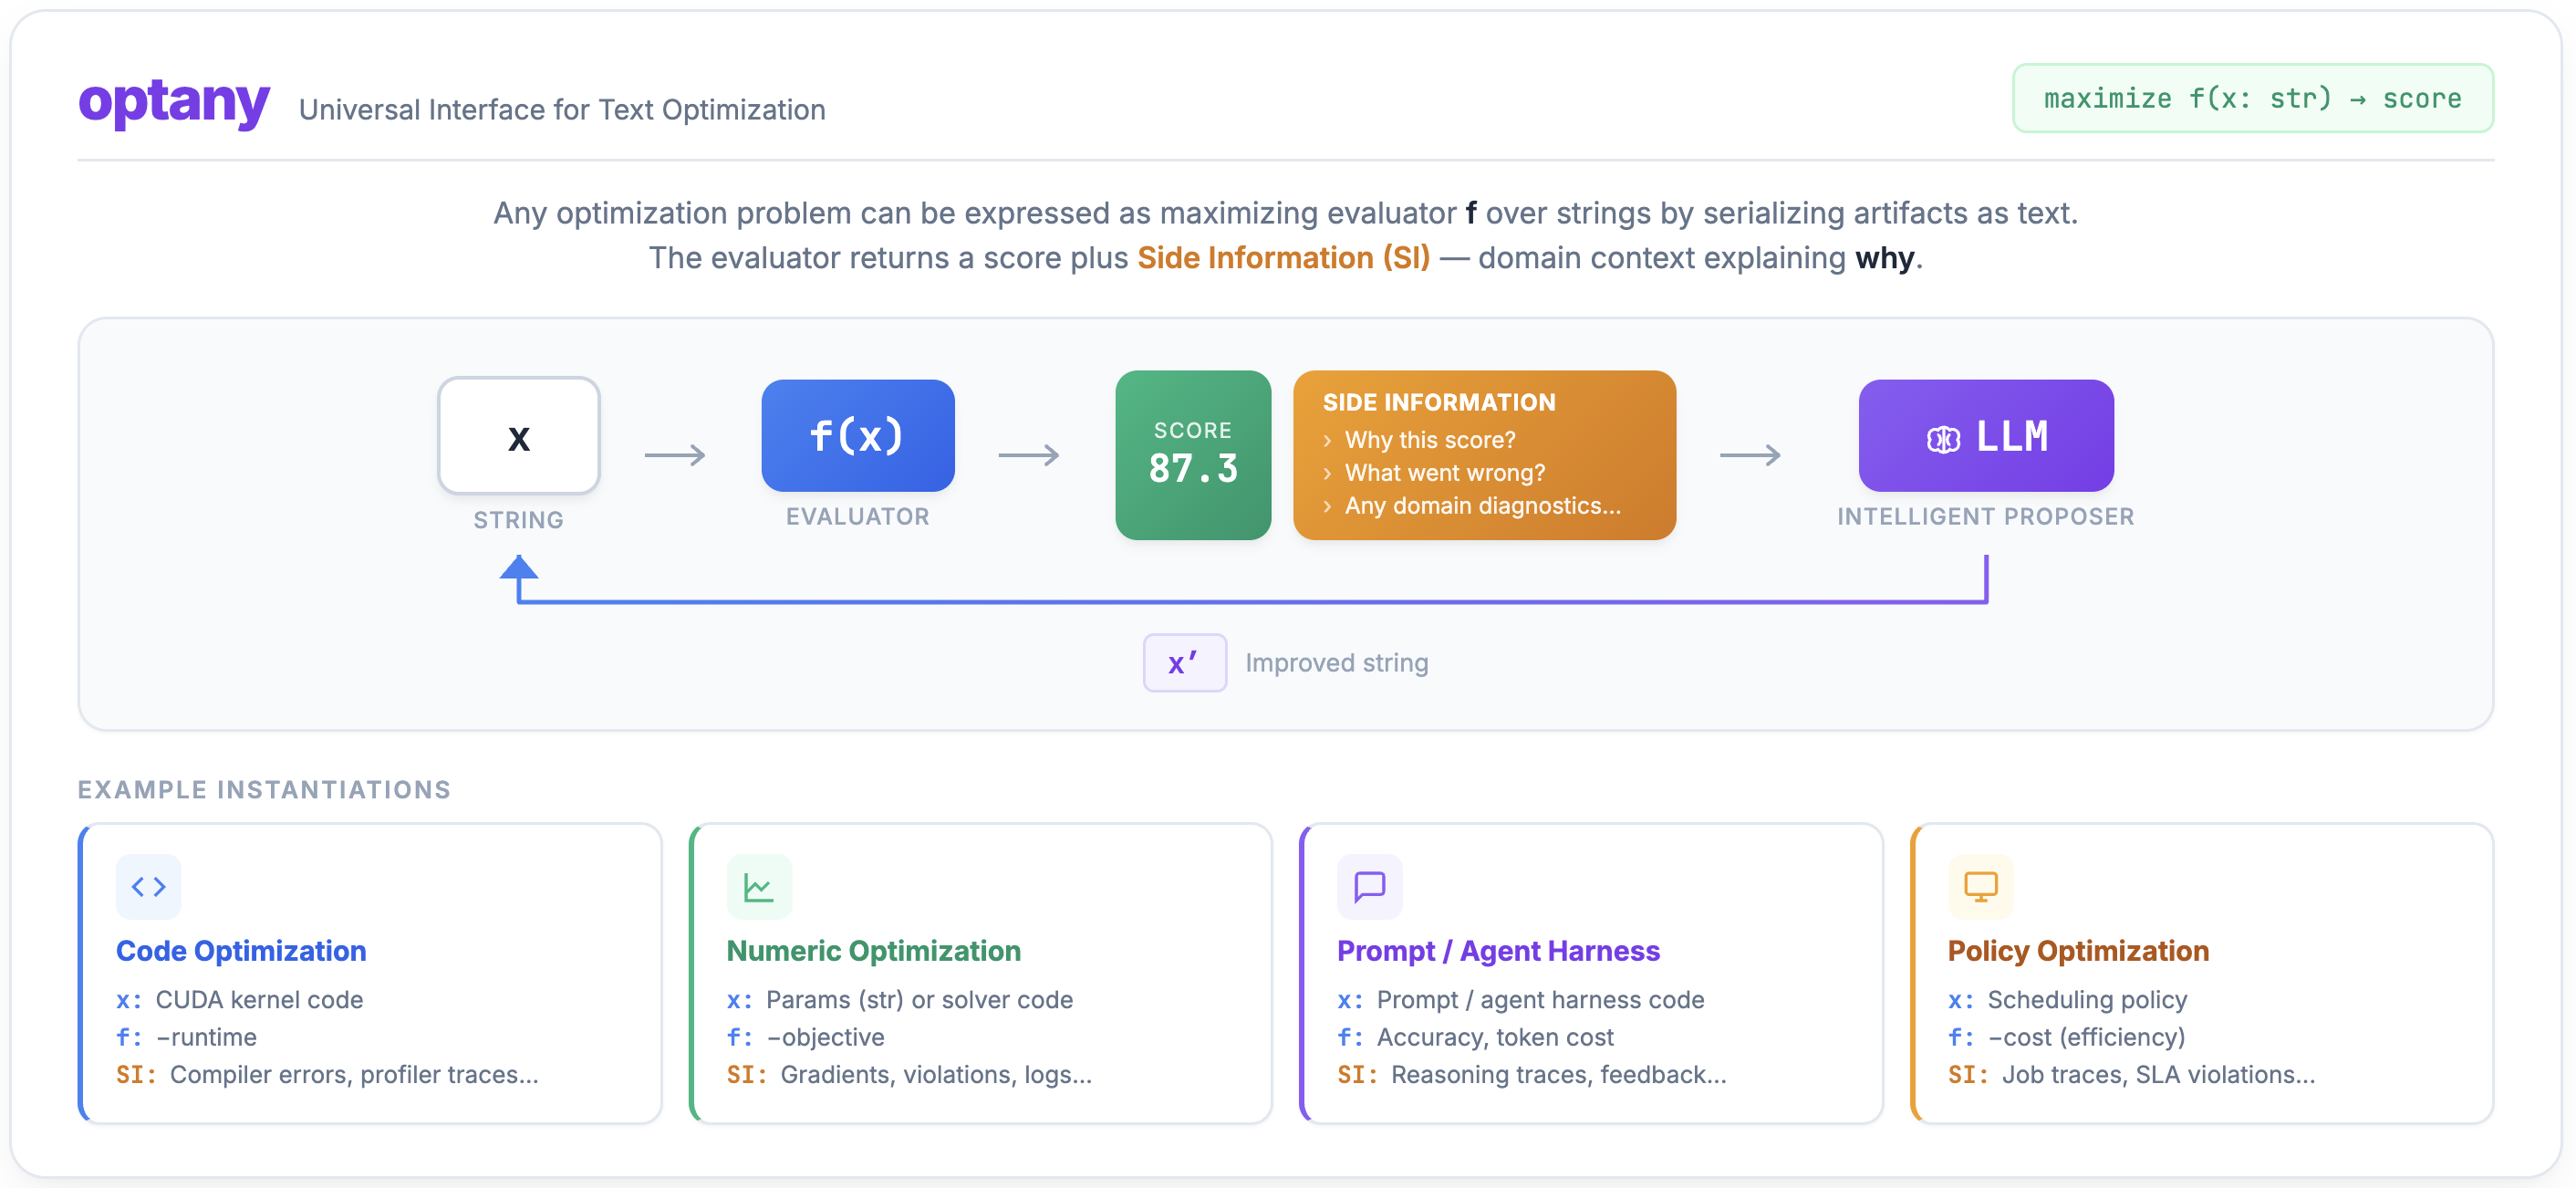
\includegraphics[width=\textwidth]{figures/header_image.png}
  \caption{The \oa{} loop: a text artifact $x$ is passed to an evaluator $f(x)$ which returns a score plus diagnostic feedback (\asi{}), which is consumed by an LLM proposer to produce an improved artifact. The same API instantiates across domains: code optimization, prompt tuning, agent architecture search, and policy discovery.}
  \Description{System diagram showing the optany loop. A string artifact is evaluated, producing scores and \asi{} feedback, which feeds into an LLM proposer that generates improved candidates. Example instantiations shown for code, prompts, agents, and policies.}
  \label{fig:overview}
\end{figure*}

%% ================================================================
\section{Introduction}\label{sec:intro}

% Large language models can serve as effective optimizers when paired with automated evaluation. FunSearch~\cite{romera2024funsearch} discovers mathematical constructions that surpass known bounds on the cap set problem. AlphaEvolve~\cite{alphaevolve2025} finds a matrix
% multiplication algorithm that improves on a 56-year-old bound and designs scheduling heuristics deployed in Google's data centers.
% GEPA~\cite{agrawal2026gepa} set the state of the art for prompt optimization across LLM benchmarks.
% These systems demonstrate remarkable results, but each has been applied to a single artifact type: code or prompts. 
Large language models can serve as effective optimizers when paired with automated evaluation. FunSearch~\cite{romera2024funsearch} evolves Python functions to discover mathematical constructions that surpass known bounds. AlphaEvolve~\cite{alphaevolve2025} extends the idea to broader code optimization, improving a 56-year-old matrix multiplication bound and designing scheduling heuristics for Google's data centers, but it operates exclusively on code artifacts, in single-task mode (one problem at a time).
GEPA~\cite{agrawal2026gepa} achieves state-of-the-art prompt optimization with generalization to unseen inputs, but is limited to prompts; MIPROv2~\cite{opsahl2024miprov2} similarly targets prompt and few-shot selection.
Despite strong results within their respective artifact types, no existing system has been applied to agent architectures, numerical optimization, or image generation, and no single system has demonstrated effectiveness across fundamentally different domains simultaneously.

% No existing system has demonstrated effectiveness across fundamentally different artifact types---agent architectures, CUDA kernels, cuda scheduling policy, numerical configurations, or Scalable Vector Graphics (SVGs).

% Recent work has demonstrated that large language models (LLMs) can serve as effective optimizers when paired with automated evaluation: FunSearch~\cite{romera2024funsearch} discovers mathematical constructions, AlphaEvolve~\cite{alphaevolve2025} designs algorithms for Google's infrastructure, and GEPA~\cite{agrawal2026gepa} sets the state-of-the-art for prompt optimization. These systems share a common insight: an LLM can read diagnostic feedback from a previous attempt, reason about its performance, and propose a targeted fix. 
% However, each framework exposes different abstractions (island topologies, mutation templates, cascade evaluators) that couple the optimization logic to framework-specific mechanisms.

We observe that a wide range of problems can be formulated as optimizing a text artifact. Whether the artifact is a CUDA kernel, a cloud scheduling policy, an agent architecture, Scalable Vector Graphics (SVGs), or a system prompt, the structure is the same: serialize the artifact as a string, evaluate it, and let an LLM propose improvements based on diagnostic feedback. This observation suggests a much simpler interface and a uniform algorithm is possible.

We present \oa{}, a declarative API that implements this insight. The user provides a seed artifact (or, in seedless mode, just a natural-language objective), an evaluator that returns a score and optional diagnostic feedback, and optionally a dataset. The system handles prompt construction, reflection, candidate selection, and search strategy. This declarative design, inspired by DSPy's~\cite{khattab2023dspy} principle of \emph{programming---not prompting}, means the same API call works whether one is optimizing an LLM prompt, an agent architecture, or an image.

Our contributions are as follows:

\begin{enumerate}[leftmargin=*,itemsep=2pt]
% \item \textbf{We show that a generic LLM-based system can match or surpass specialized systems across six domains.} We show that the same simple abstraction enables expressing diverse problems as text optimization problems, and discover agent architectures that nearly triple ARC-AGI accuracy (32.5\% $\to$ 89.5\%), discover scheduling algorithms that cut cloud costs by 40\%, generate CUDA kernels where 87\% match or beat PyTorch baselines, and outperform AlphaEvolve's solution on circle packing. This establishes that LLM-based text optimization is a broadly effective paradigm, not limited to a single niche.
\item \textbf{A single LLM-based Text Optimization system matches or surpasses domain-specific tools across six fundamentally different domains.} We are the first to show that a single system (our proposed \oa{}) can optimize code, prompts, agent architectures, numerical configurations, and images, achieving state-of-the-art results in each. Our system discovers agent architectures that nearly triple ARC-AGI accuracy (32.5\% $\to$ 89.5\%), finds scheduling algorithms that cut cloud costs by 40\%, generates CUDA kernels where 87\% match or beat PyTorch baselines, create custom solver code matching and outperforming Optuna in numerical optimization, and outperforms AlphaEvolve's solution on circle packing. This establishes LLM-based text optimization as a general-purpose problem-solving paradigm, not limited to code or prompts.

% \item \textbf{We unify three optimization modes---single-task, multi-task, and generalization--- under one interface.} Prior frameworks (AlphaEvolve~\cite{alphaevolve2025}, OpenEvolve~\cite{openevolve2025}, ShinkaEvolve~\cite{shinkaevolve2025}) operate exclusively in single-task mode: optimize one artifact for one problem. \oa{} additionally supports \emph{multi-task search}, where solving a batch of related problems enables cross-transfer of optimization patterns, and \emph{generalization}, where the optimized artifact must perform well on unseen examples. These modes enable optimization tasks that prior frameworks cannot directly express, such as optimizing coding agent skills that transfer across models (\S\ref{sec:skills}), discovering agent architectures from scratch (\S\ref{sec:arc}), and learning prompts that generalize to unseen test sets (\S\ref{sec:aime}).
% \item \textbf{Three optimization modes---single-task, multi-task, and generalization--- unified under one interface.} Code-evolution frameworks (AlphaEvolve~\cite{alphaevolve2025}, OpenEvolve~\cite{openevolve2025}, ShinkaEvolve~\cite{shinkaevolve2025}) support only single-task mode: one artifact for one problem. Prompt optimizers (GEPA~\cite{agrawal2026gepa}, MIPROv2~\cite{opsahl2024miprov2}) primarily support generalization to unseen inputs, but only for prompts. No prior system supports \emph{multi-task search}, where solving related problems together enables cross-transfer of optimization patterns. \oa{} unifies all three modes under one interface: multi-task search on CUDA kernels consistently outperforms independent single-task optimization given equivalent per-problem budget (\S\ref{sec:multi-ablation}), and generalization mode extends beyond prompts to agent architectures (\S\ref{sec:arc}) and scheduling policies (\S\ref{sec:cloud}).
\item \textbf{Three optimization modes---single-task, multi-task, and generalization---unified under one interface, including the first multi-task mode.} Existing LLM-evolution systems each support exactly one mode. AlphaEvolve~\cite{alphaevolve2025}, OpenEvolve~\cite{openevolve2025}, and ShinkaEvolve~\cite{shinkaevolve2025} operate in single-task mode: optimizing one code artifact for one problem at a time. GEPA~\cite{agrawal2026gepa} and MIPROv2~\cite{opsahl2024miprov2} operate in generalization mode: optimizing a prompt to perform well on unseen inputs, but only for prompts. No prior system supports \emph{multi-task search}, where solving a batch of related problems together enables cross-transfer of discovered optimization patterns. \oa{} unifies all three modes under one interface: multi-task search on CUDA kernels outperforms independent single-task optimization given equivalent per-problem budget (\S\ref{sec:multi-ablation}), and generalization extends beyond prompts to agent architectures (\S\ref{sec:arc}) and scheduling policies (\S\ref{sec:cloud}). All optimization modes are expressed through the same \oa{} API.

\item \textbf{Side information as a first-class evaluator contract.} Prior frameworks support diagnostic feedback through ad-hoc, framework specific mechanisms. \oa{} elevates it to a uniform API contract: any diagnostic---stack traces, profiler data, rendered images, structured error reports---flows to the proposer through one interface. Ablations show that side information yields 4-6$\times$ faster convergence and a 3.8-point improvement in final test performance versus score-only feedback (\S\ref{sec:asi-ablation}).
\end{enumerate}

We achieve these results by extending the Pareto-based search of~\citet{agrawal2026gepa} (originally studied only for prompt optimization) to arbitrary text artifacts, adding single-task and multi-task modes. Candidates are selected based on per-example or per-metric Pareto dominance rather than aggregate scores, preserving complementary strengths across iterations. Table~\ref{tab:comparison} provides a detailed comparison.

We evaluate \oa{} across six primary domains spanning all three optimization modes (Table~\ref{tab:summary}), with two additional domains (blackbox mathematical optimization and 3D modeling) in the appendix as preliminary demonstrations. Key results include: (i) evolved agent architectures nearly triple Gemini Flash's ARC-AGI accuracy (32.5\% $\to$ 89.5\%); (ii) discovered cloud scheduling algorithms cut costs by up to 40\%; (iii) 87\% of generated CUDA kernels match or beat PyTorch baselines from KernelBench, with multi-task mode outperforming dedicated single-task optimization; (iv) prompt optimization improves GPT-4.1-mini's AIME-2025 accuracy from 46.67\% to 60.00\%; and (v) our circle packing solution outperforms AlphaEvolve's published one. Ablations show that side information yields 4-6$\times$ faster convergence and +3.8 test points over score-only feedback.

%% ================================================================
\section{Related Work}\label{sec:related}

\paragraph{LLM-based program evolution.}
AlphaEvolve~\cite{alphaevolve2025} pioneered the LLM-evolution paradigm, using Gemini models with island-based MAP-Elites~\cite{mouret2015mapelites} to discover algorithms for Google's infrastructure. OpenEvolve~\cite{openevolve2025} provides an open-source reimplementation with model-agnostic support. ShinkaEvolve~\cite{shinkaevolve2025} extends the paradigm with novelty-based rejection sampling for sample efficiency and adaptive LLM ensemble selection for diversity. FunSearch~\cite{romera2024funsearch} applies evolutionary LLM search to mathematical discovery. EvoPrompting~\cite{chen2024evoprompting} evolves code for neural architecture search. All operate exclusively in single-task mode and expose framework-specific abstractions (island topologies, prompt samplers, evolve-block markers). \oa{} strips the interface to its declarative essence, adds multi-task and generalization modes, and elevates diagnostic feedback to a first-class API concept.

\paragraph{Prompt optimization.}
GEPA~\cite{agrawal2026gepa} combines reflective mutation with a Pareto-based search technique for prompt optimization, outperforming both MIPROv2~\cite{opsahl2024miprov2} and GRPO~\cite{shao2024grpo}. \oa{} uses GEPA's evolutionary search algorithm as the optimization backend, extending it beyond prompts to arbitrary text artifacts. Other prompt optimization methods include OPRO~\cite{yang2024opro}, APE~\cite{zhou2023ape}, ProTeGi~\cite{pryzant2023prompt}, and PromptBreeder~\cite{fernando2024promptbreeder}. TextGrad~\cite{yuksekgonul2024textgrad} uses LLM-generated ``gradients'' for text optimization.

\paragraph{LLM self-improvement and reflection.}
Reflexion~\cite{shinn2023reflexion} uses verbal reinforcement for agent self-correction. Self-Refine~\cite{madaan2023selfrefine} applies iterative self-feedback. Evolution through Large Models~\cite{lehman2022evolution} explores LLMs as mutation operators. \oa{}'s \asi{} mechanism generalizes these ideas by making diagnostic feedback a declarative evaluator contract rather than a hardcoded self-critique.

\paragraph{Agent architecture search.}
ADAS~\cite{hu2024automated} and AFlow~\cite{zhang2024aflow} search over agent architectures. \oa{}'s generalization mode subsumes these as special cases: the artifact is the agent code, the evaluator runs it on tasks, and the system evolves both architecture and prompts jointly.

%% ================================================================
\section{The \oa{} API}\label{sec:api}

\subsection{Core Interface}

At its simplest, \oa{} requires a seed artifact and an evaluator. The evaluator takes a candidate string and returns a score (higher is better) alongside an optional Side Information (\asi{}) dictionary containing diagnostic feedback the proposer reads during reflection:

\begin{lstlisting}
import optany as oa

def evaluate(candidate: str) -> tuple[float, dict]:
    result = execute_code(candidate)
    return result.score, {
        "Error": result.stderr,
        "Output": result.stdout,
        "Runtime": f"{result.time_ms:.1f}ms",
    }

result = oa.optany(
    seed_candidate="<your artifact>",
    evaluator=evaluate,
)
\end{lstlisting}

\asi{} can include open-ended text, structured data, multiple sub-scores, or images (via \texttt{oa.Image}) for Vision-capable LLMs (VLM).

The full \oa{} signature is:
\begin{lstlisting}
def optany(
    seed_candidate=None,   # Starting artifact
    evaluator=...,         # fn(candidate) -> Score + SI
    dataset=None,          # Training examples
    valset=None,           # Validation set
    objective=None,        # Natural language goal
    background=None,       # Domain knowledge
    config=None,           # Engine settings
) -> OptimizationResult:
\end{lstlisting}

Specifically, \oa{} doesn't require mutation prompts, task-specific templates, island configurations, or \texttt{EVOLVE-BLOCK} markers (all common in prior frameworks). The user declares the \emph{what} (artifact, evaluator, domain knowledge), and \oa{}, through its optimization backends, handles the \emph{execution}.

\paragraph{Seedless mode.} In domains where providing even a starting artifact is difficult, or where writing even a bad seed requires domain expertise (e.g., 3D modeling), the user can just provide a natural-language \texttt{objective} as an argument in place of the \texttt{seed\_candidate} argument and the LLM bootstraps the first candidate from scratch. Seedless mode makes the system accessible to users who can \emph{specify} what they want but not \emph{implement} it. Appendix~\ref{app:unicorn} demonstrates it on a 3D modeling task.

\subsection{Three Optimization Modes}\label{sec:modes}

Which mode is active depends solely on whether \texttt{dataset} and \texttt{valset} are provided:

\paragraph{Single-Task Search.} No dataset. The candidate \emph{is} the solution; the evaluator scores it directly. This is the mode that AlphaEvolve and OpenEvolve operate in. Example: in circle packing (\S\ref{sec:circle}), the artifact is the packing algorithm and the evaluator returns the packing score plus geometric diagnostics.

\paragraph{Multi-Task Search.} A \texttt{dataset} of related tasks is provided; insights from solving one help solve the others. Example: in CUDA kernel generation (\S\ref{sec:cuda}), each task is a PyTorch operation to accelerate. Multi-task mode discovers optimization patterns that transfer across problems, converging faster and solving more problems than single-task runs (\S\ref{sec:multi-ablation}). No prior LLM-evolution framework supports this mode.

\paragraph{Generalization.} Both \texttt{dataset} and \texttt{valset} are provided; the optimized artifact must perform well on unseen examples. This is the mode that GEPA's prompt optimization~\cite{agrawal2026gepa} operates in. \\ \oa{} generalizes the pattern to any text artifact. Example: in agent architecture discovery (\S\ref{sec:arc}), the artifact is the entire agent, and it must generalize to unseen ARC-AGI puzzles.

\begin{table}[t]
\caption{Summary of experimental results across six domains. ``Mode'' indicates which optimization paradigm is used: S = single-task search, M = multi-task search, G = generalization. All results use \oa{} with the indicated proposer LLM.}
\label{tab:summary}
\small
\begin{tabular}{@{}llllr@{}}
\toprule
\textbf{Domain} & \textbf{Mode} & \textbf{Proposer} & \textbf{Key Result} \\
\midrule
Agent Skills (\S\ref{sec:skills}) & G & Claude Opus 4.6 & 100\% pass rate (+20.7pp) \\
Cloud Sched. (\S\ref{sec:cloud}) & G & Gemini 3 Pro & 40.2\% cost savings \\
ARC-AGI (\S\ref{sec:arc}) & G & Gemini 3 Flash & 89.5\% test (+57pp) \\
AIME Prompts (\S\ref{sec:aime}) & G & GPT-5 & 60.0\% test (+13.3pp) \\
CUDA Kernels (\S\ref{sec:cuda}) & M & GPT-5 & 87\% match baseline \\
Circle Pack. (\S\ref{sec:circle}) & S & GPT-5 & Beats AlphaEvolve \\
Math Opt. (\S\ref{app:optuna}) & S & GPT-5 & Wins 7/10 vs Optuna \\
3D Modeling (\S\ref{app:unicorn}) & S & Cloud Opus 4.6 & Generates a 3D unicorn \\
\bottomrule
\end{tabular}
\end{table}


%% ================================================================
\section{Method}\label{sec:method}

\oa{} currently extends and manages information atop GEPA~\cite{agrawal2026gepa}, an algorithm originally studied primarily in the context of prompt optimization and code search, as the optimization backend.
The system overview is shown in Figure~\ref{fig:overview}. We describe the two mechanisms that underpin its effectiveness and contrast \oa{} with prior frameworks.

\begin{table}[t]
\caption{Comparison of \oa{} with prior LLM-evolution frameworks. Only \oa{} supports multi-task search and generalization modes, and provides diagnostic feedback as a first-class API concept.}
\label{tab:comparison}
\small
\resizebox{\columnwidth}{!}{%
\begin{tabular}{@{}lcccc@{}}
\toprule
\textbf{Feature} & \rotatebox{70}{\textbf{AlphaEv.}} & \rotatebox{70}{\textbf{OpenEv.}} & \rotatebox{70}{\textbf{ShinkaEv.}} & \rotatebox{70}{\textbf{\oa{}}} \\
\midrule
Single-task search & \checkmark & \checkmark & \checkmark & \checkmark \\
Multi-task search & & & & \checkmark \\
Generalization & & & & \checkmark \\
\asi{} as API contract & & & & \checkmark \\
Image feedback & & & & \checkmark \\
Declarative interface & & & & \checkmark \\
No mutation templates & & & & \checkmark \\
Open-source & & \checkmark & \checkmark & \checkmark \\
\bottomrule
\end{tabular}%
}
\end{table}

\subsection{Problem Formulation}\label{sec:formulation}

    We formalize the text optimization problem as follows. Let $\mathcal{X}$ denote the space of text artifacts (strings). An evaluator $f:\mathcal{X}\times\mathcal{E} \cup \{\bot\} \to \mathbb{R}\times\mathcal{I}$ maps an artifact $x\in\mathcal{X}$ and an (optional) example $e\in\mathcal{E} \cup \{\bot\} $ to a score $s(x,e)\in\mathbb{R}$ and side information $\iota(x,e)\in\mathcal{I}$, i.e., $f(x,e)=(s(x,e),\iota(x,e))$. The three modes correspond to:

\textbf{Single-task search:} $\mathcal{E}=\emptyset$; maximize $s(x)$ directly. The artifact \emph{is} the solution (e.g., a packing algorithm).

\textbf{Multi-task search:} Given a dataset $\mathcal{D}=\{e_1,\ldots,e_n\}$ of related problems, find an artifact $x\in\mathcal{X}$ (e.g., a kernel-generation prompt) maximizing $\frac{1}{n}\sum_{i=1}^{n} s(x,e_i)$. Cross-transfer arises because the Pareto frontier preserves patterns that work across problems.

\textbf{Generalization:} Given a training set $\mathcal{D}_{\text{train}}$ and a validation set $\mathcal{D}_{\text{val}}=\{e^{\text{val}}_1,\ldots,e^{\text{val}}_k\}$, find an artifact $x\in\mathcal{X}$ maximizing $\frac{1}{k}\sum_{j=1}^{k} s\!\left(x,e^{\text{val}}_j\right)$. Search uses feedback from $\mathcal{D}_{\text{train}}$, while $\mathcal{D}_{\text{val}}$ measures generalization to unseen examples. This generalizes classical machine learning: the artifact may be a prompt, an agent, or a policy.

\subsection{Side Information (\asi{})}\label{sec:asi}

Popularly used numerical optimization methods like gradient descent reduce all diagnostic context to a single scalar. The optimizer knows \emph{that} a candidate failed, but not \emph{why}. For example, one cannot show a Bayesian optimizer a stack trace. LLM-evolution frameworks changed this by feeding execution results into LLM proposers, but when an LLM reads a compiler error, diagnoses a logic bug, and proposes a targeted fix, the process is closer to an engineer iterating on a prototype than to blind evolution.

\oa{} leans into this by making diagnostic feedback a first-class part of the evaluator contract. The evaluator returns both a score and a \texttt{side\_info} dictionary containing any diagnostic the evaluator can produce:

\begin{itemize}[leftmargin=*,itemsep=1pt]
  \item \textbf{Text:} compiler errors, runtime exceptions, profiler summaries, natural-language critiques.
  \item \textbf{Structured data:} per-test-case results, sub-scores for multiple objectives, execution traces.
  \item \textbf{Images:} rendered SVGs, 3D model screenshots, or chart visualizations, enabling VLM proposers to \emph{see} what they are improving.
\end{itemize}

\asi{} is the text-optimization analogue of the gradient. Where gradients tell a numerical optimizer which direction to move, \asi{} can tell the LLM proposer \emph{why} a candidate failed and \emph{how} to fix it. During a dedicated reflection step, the proposer reasons over this signal to diagnose failures and propose targeted improvements.

Prior frameworks expose feedback through framework-specific mechanisms; \asi{} provides a uniform interface that makes it trivial to surface any diagnostic. The key design choice is that \asi{} is \emph{opt-in but zero-friction}: evaluators that return only a score work fine, and existing \texttt{print()} statements can be captured automatically via \texttt{capture\_stdio=True}.

\subsection{Pareto-Based Search}\label{sec:pareto}

Even when optimizing a single objective, evaluating candidates across multiple examples or metrics produces richer signal than a scalar aggregate. The naive approach collapses that signal into one average score and always selects the top candidate. This stalls fast: averaging hides which aspects are strong and which are weak, and the proposer tries to improve everything at once.

\oa{} does two things differently. First, it tracks scores per task (from \texttt{dataset}) or per metric (from sub-scores in \asi{}) individually and maintains a \textbf{Pareto frontier}: any candidate that is the best at \emph{something} survives, even if its average is suboptimal. Second, each reflection step shows the proposer a minibatch of just 2--3 examples instead of all of them, enabling focused, targeted improvements on that subset.

Over iterations, the frontier accumulates complementary strengths. Candidates that excel at different tasks are preserved and their strategies recombined. This mechanism also powers multi-task search: when optimizing across related problems, the frontier preserves candidates that excel on different tasks, and strategies discovered for one problem transfer to others (\S\ref{sec:multi-ablation}).

\paragraph{Candidate selection.} Following GEPA~\cite{agrawal2026gepa}, candidates are selected for mutation in proportion to how often they appear on the Pareto front. Let $J$ index the objectives used to form the Pareto scores (e.g., per-example tasks, per-metric scores, or both). Each candidate $\Phi$ induces a score $s_j(\Phi)$ for every $j\in J$. Let $\mathcal{P}$ denote the set of Pareto-nondominated candidates under these objectives. For each objective $j\in J$, let $\mathcal{B}[j]$ be the set of candidates in $\mathcal{P}$ that achieve the best score on $j$. We sample candidates with probability proportional to $|\{j\in J : \Phi \in \mathcal{B}[j]\}|$, focusing exploration on broadly effective solutions.

\paragraph{Reflection and mutation.} Given a selected candidate $\Phi$ and a minibatch $\mathcal{M}$ of examples, the system executes $\Phi$ on $\mathcal{M}$, collects scores and \asi{}, and presents them to the proposer LLM in a structured reflection prompt. The proposer diagnoses failures using the \asi{} and produces an updated artifact $\Phi'$. If $\Phi'$ improves on the minibatch, it is fully evaluated and added to the candidate pool.


%% ================================================================
\section{Experiments}\label{sec:experiments}

We evaluate \oa{} across six domains spanning all three optimization modes. For each, we describe the artifact, evaluator, \asi{} design, and results. We then present ablation studies on multi-task search (\S\ref{sec:multi-ablation}) and \asi{} (\S\ref{sec:asi-ablation}).
Optimized solutions are presented in the Appendix \ref{app:discovered_solutions}.

\subsection{Coding Agent Skills (Generalization)}\label{sec:skills}

\textbf{Setup.} Skills are natural-language instructions and best practices for working with a specific codebase. The evaluator runs a coding agent on repository tasks and scores whether it resolves them; the optimized skills must generalize to unseen tasks. We optimize skills for the Bleve search library and evaluate transfer to Claude Code with both Haiku 4.5 and Sonnet 4.5.

\textbf{\asi{} design.} The evaluator returns task descriptions, agent traces (tool calls, code edits, errors), test outcomes, and resolution time.

\textbf{Results.} Optimized skills boost Haiku 4.5's pass rate from 79.3\% to 98.3\% and Sonnet 4.5's from 94.8\% to 100\%, while cutting resolution time by 47\% (Figure~\ref{fig:skills}). Critically, skills discovered for one model transfer effectively to another without reoptimization, demonstrating the generalization mode's ability to learn model-agnostic repository knowledge.

\begin{figure}[t]
  \centering
  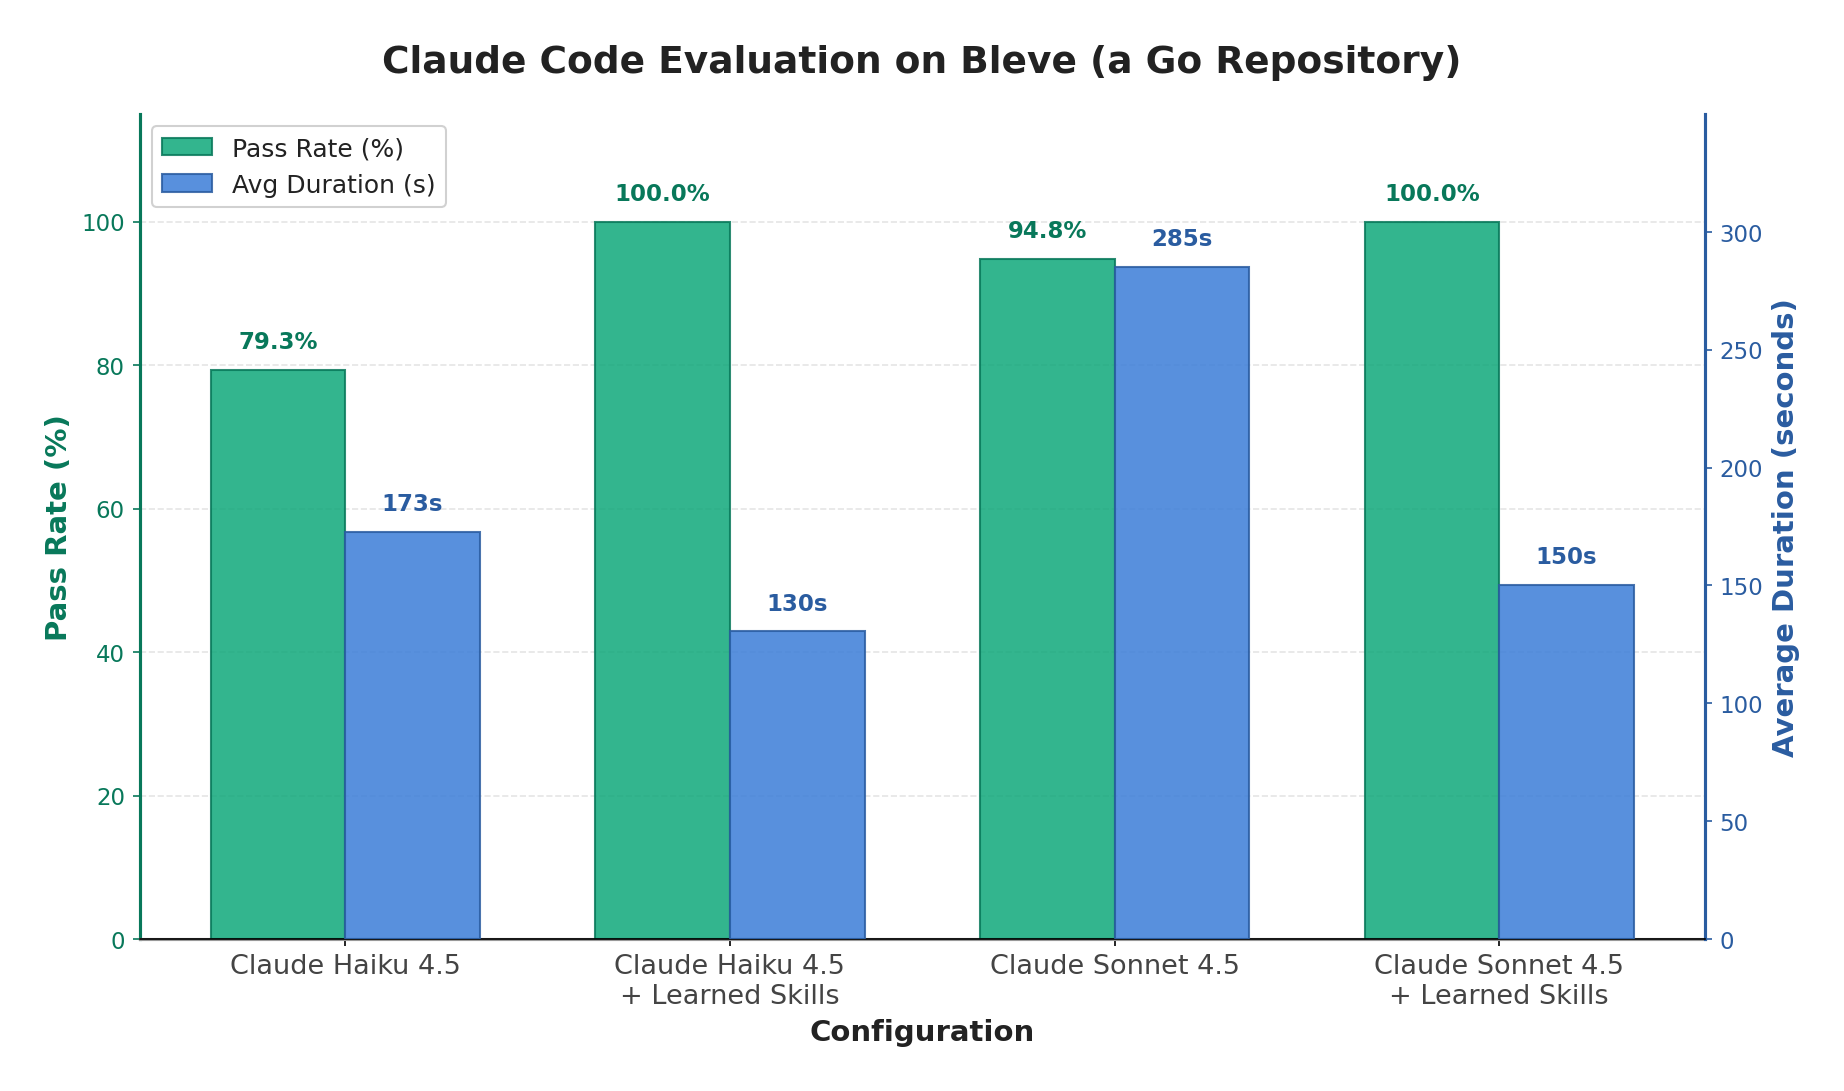
\includegraphics[width=\columnwidth]{figures/bleve_comparison_plot.png}
  \caption{Claude Code on the Bleve repository. Optimized skills boost pass rates to near-perfect while reducing resolve time by 47\%. Skills transfer across models without reoptimization.}
  \Description{Bar chart showing pass rates: Haiku 4.5 79.3\% (173s), Haiku 4.5 + Skills 98.3\% (142s), Sonnet 4.5 94.8\% (285s), Sonnet 4.5 + Skills 100\% (169s).}
  \label{fig:skills}
\end{figure}


\subsection{Cloud Scheduling Algorithms (Generalization)}\label{sec:cloud}

\textbf{Setup.} We optimize two cloud infrastructure algorithms from the ADRS benchmark. \textbf{CloudCast} discovers broadcast routing strategies for multi-cloud data transfer, minimizing data egress cost. \textbf{Can't Be Late} learns scheduling policies deciding when to use cheap preemptible \texttt{SPOT} instances versus reliable \texttt{ON\_DEMAND} instances to meet deadlines. Both use generalization mode with training/validation splits over infrastructure scenarios.

\textbf{\asi{} design.} For CloudCast: per-partition routing decisions, edge utilizations, cost breakdowns. For Can't Be Late: spot-availability patterns, instance-usage timelines, segment counts (\texttt{SPOT} vs \\ \texttt{ON\_DEMAND} vs restarts).

\textbf{Results.} CloudCast achieves 40.2\% cost savings over Dijkstra routing (Figure~\ref{fig:clouda}), evolving from a baseline shortest-path algorithm to a provider-aware Steiner tree approach that jointly optimizes for egress cost and transfer latency. Can't Be Late achieves 7.8\% cost savings (Figure~\ref{fig:cloudb}), evolving a simple deadline-check heuristic into an adaptive strategy with state tracking for spot-unavailability patterns, break-even switching cost analysis, and graduated decision thresholds based on slack ratio.
Both results top the ADRS leaderboard, outperforming OpenEvolve, ShinkaEvolve, and expert-designed heuristics. The evolved artifacts are qualitatively different from their seeds: CloudCast discovers provider-aware routing with Steiner tree relaxation (concepts not present in the Dijkstra seed), while Can't Be Late learns to track persistent spot unavailability and compute overhead-aware switching costs (behaviors absent from the greedy seed).

\begin{figure}[t]
  \centering
  \begin{subfigure}[b]{0.95\columnwidth}
    
\includegraphics[width=\textwidth]{cais_submission/figures/cloudcast.png}
    \caption{CloudCast: 40.2\% cost savings.}
    \label{fig:clouda}
  \end{subfigure}
  
  \begin{subfigure}[b]{0.95\columnwidth}
    
\includegraphics[width=\textwidth]{cais_submission/figures/cantbelate.png}
    \caption{Can't Be Late: 7.8\% savings.}
    \label{fig:cloudb}
  \end{subfigure}
  \caption{Optimization trajectories for cloud scheduling. Both use generalization mode with train/val splits over infrastructure scenarios.}
  \Description{Two line charts showing optimization trajectories. CloudCast reaches 40.2\% test savings. Can't Be Late reaches 7.8\% test savings.}
  \label{fig:cloud}
\end{figure}


\subsection{ARC-AGI Agent Architecture (Generalization)}\label{sec:arc}
% TODO: Add the ARC-AGI architecture diagram
\textbf{Setup.} Rather than optimizing a prompt, we optimize the \emph{entire agent system}: code, sub-agent architecture, control flow, helper functions, and prompts are all treated as a single text artifact. The optimization objective is for the artifact to generalize to unseen ARC-AGI~\cite{chollet2019arc} puzzles.

\textbf{\asi{} design.} Training/test grid examples, per-puzzle scores, internal model outputs, LLM costs, error tracebacks, and code execution results.

\textbf{Results.} Using Gemini 3 Flash as both the proposer and the underlying agent model, \oa{} starts for a naive 10-line agent seed (one LLM call) and iteratively designs it into a 300+ line system consisting of 4 components along with fallbacks. The test accuracy improves from 32.5\% to \textbf{89.5\%}, a 57 percentage point gain (Figure~\ref{fig:arc}). The optimized architecture implements a 4-stage pipeline: (1) rule induction via pattern analysis, (2) code generation with \texttt{exec()}-based verification, (3) iterative debugging with up to 2 fix attempts, and (4) structured fallback from code-first to direct LLM prediction. This represents a qualitative leap: the system discovers architectural patterns (verify-then-fallback, iterative refinement) that typically require manual engineering iterations.

\begin{figure}[t]
  \centering
  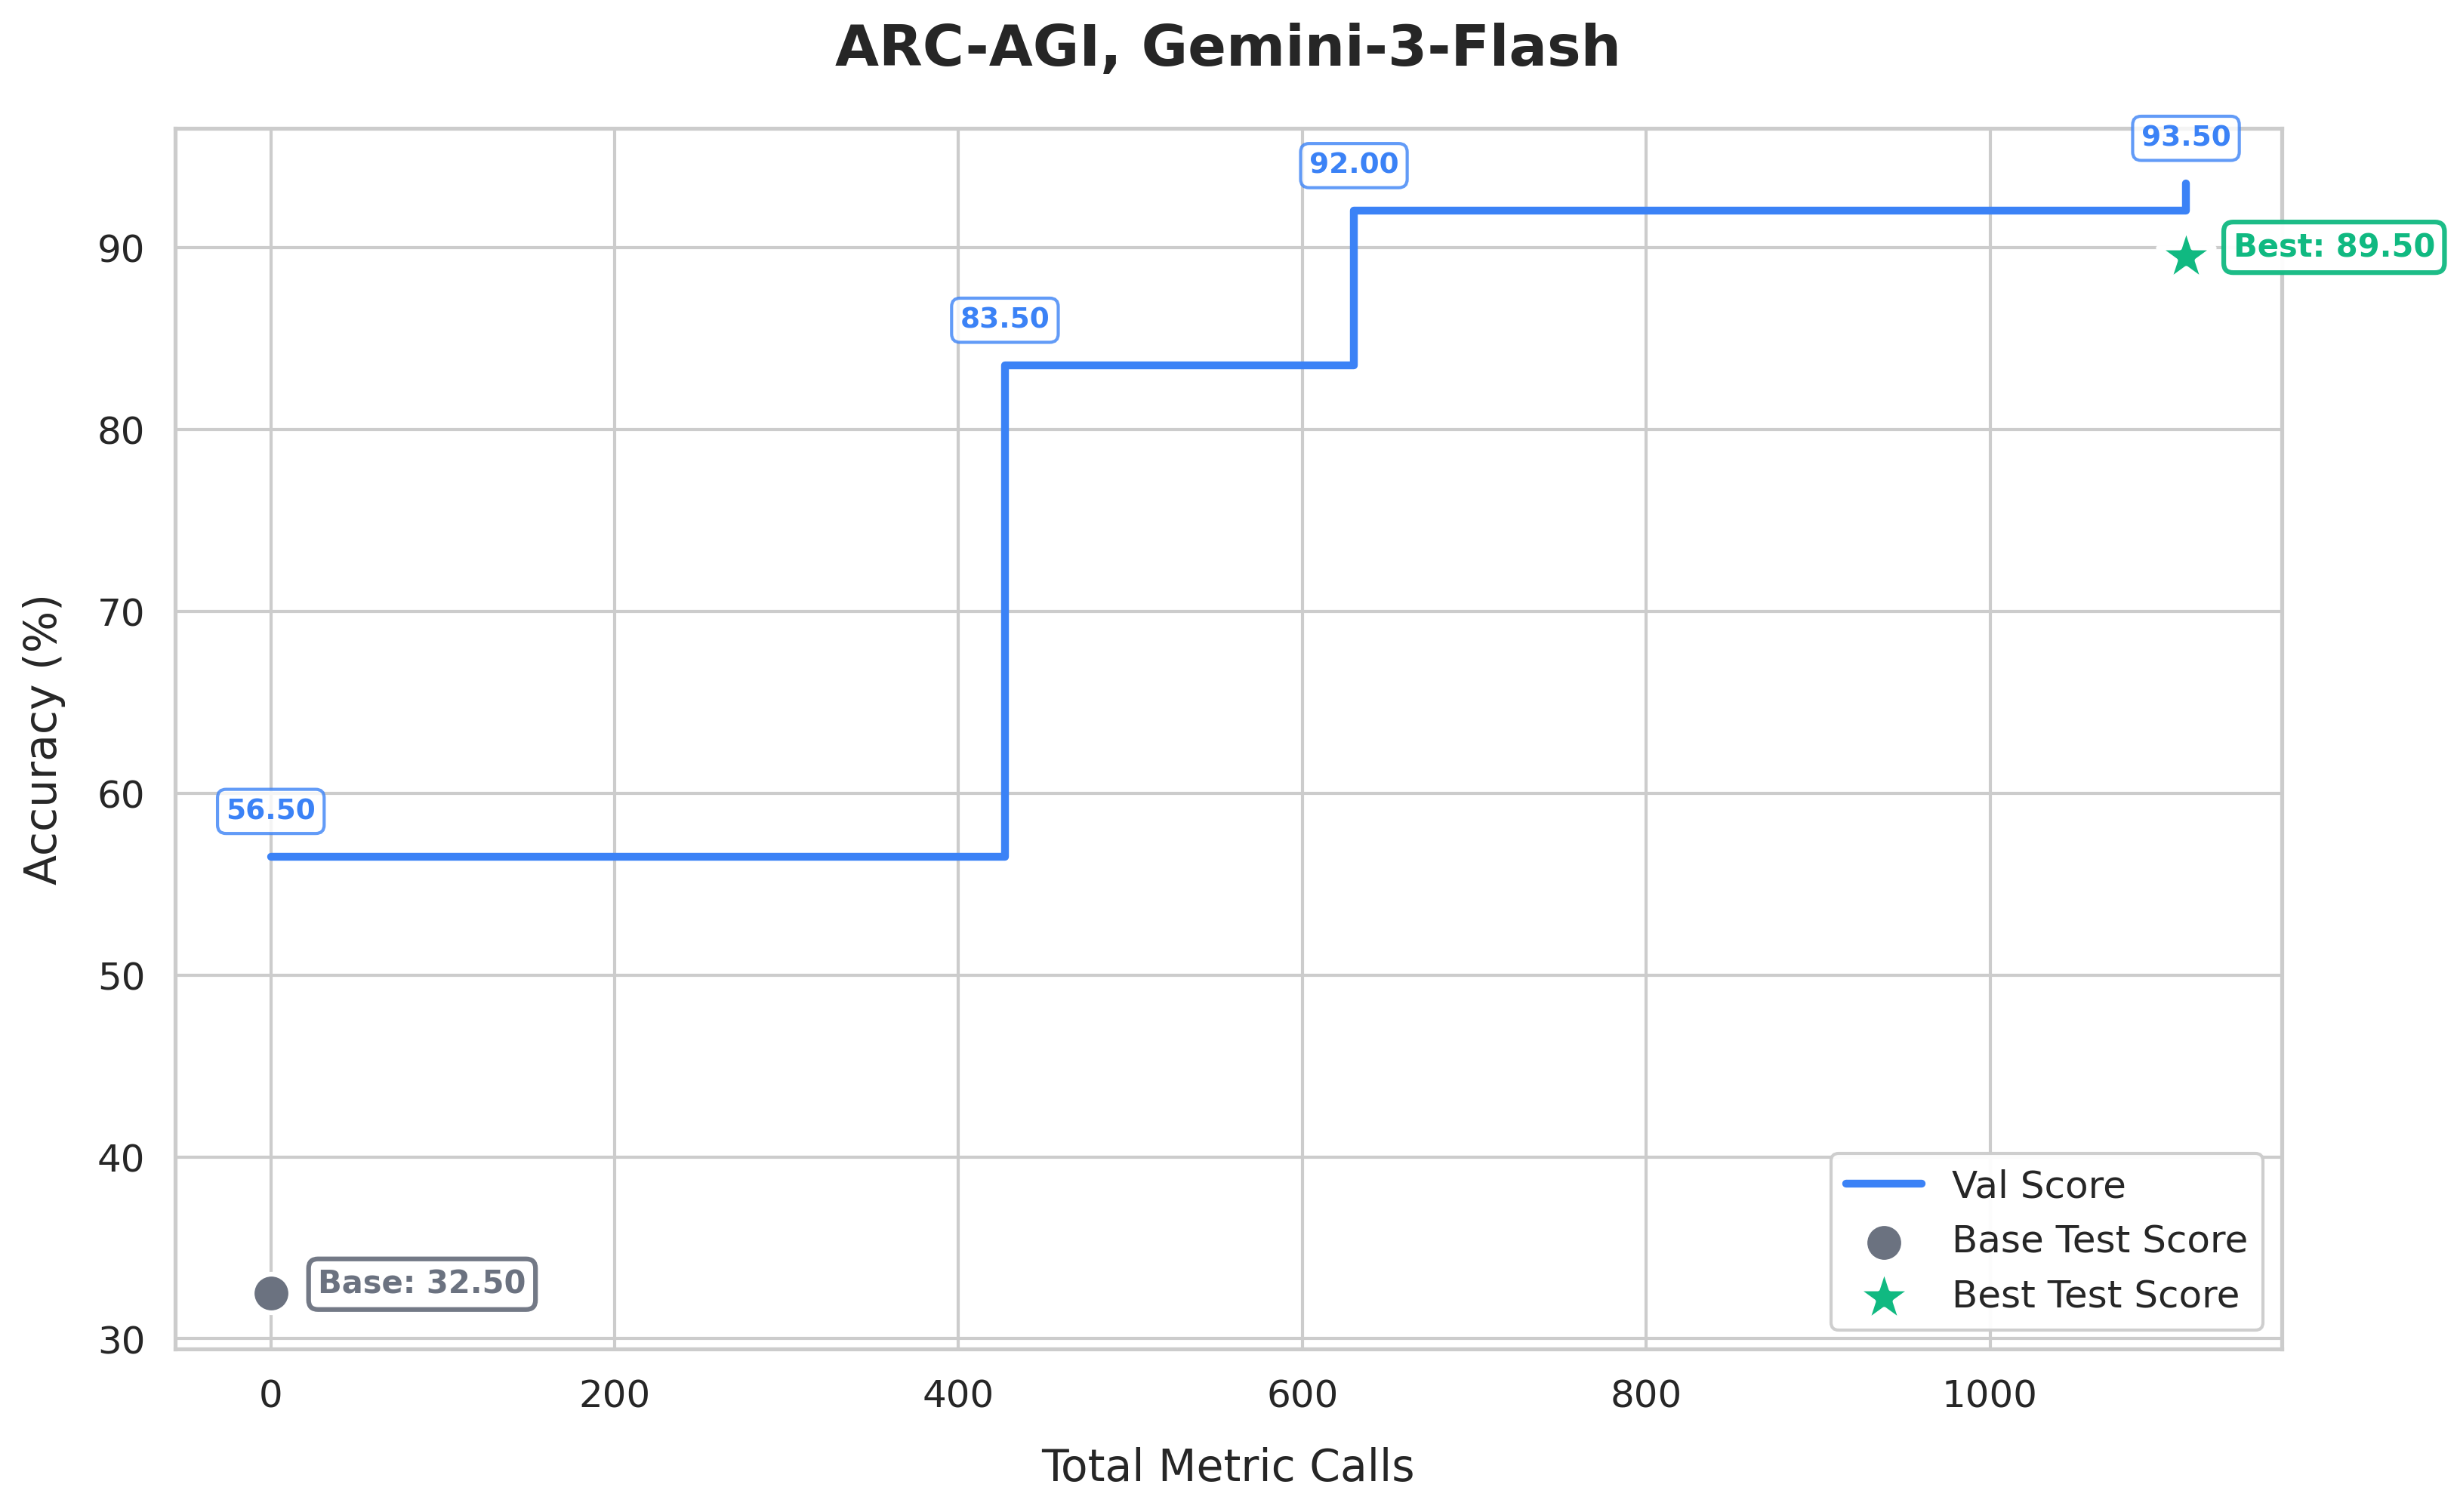
\includegraphics[width=\columnwidth]{figures/arc_agi_trajectory.png}
  \caption{ARC-AGI agent architecture evolution with Gemini 3 Flash. Validation accuracy reaches 93.5\%; test accuracy improves from 32.5\% to 89.5\%.}
  \Description{Line chart showing validation accuracy improving from about 56\% to 93.5\% over metric calls. Base test 32.5\%, best test 89.5\%.}
  \label{fig:arc}
\end{figure}


\subsection{AIME Prompt Optimization (Generalization)}\label{sec:aime}


\textbf{Setup.} We optimize a system prompt for GPT-4.1-mini on AIME (American Invitational Mathematics Examination) competition problems. Training uses AIME 2022--2024; testing uses AIME 2025.


% \begin{figure}[t]
\begin{promptbox}[Optimized Prompt for AIME]
Solve the math problem carefully and thoroughly. Your goal is to produce a correct,
well‑structured solution that leads unambiguously to the requested final result.

Follow these rules:

1. Restate the problem briefly in your own words.

2. Set up notation and equations cleanly before manipulating them.
   - Define variables explicitly.
   - State all constraints (e.g., integrality, ranges, geometric conditions) before
     using them.

3. Show clear, logically ordered reasoning.
   - Justify each important algebraic or geometric step.
   - When you split into cases, state why each case is necessary and what assumptions
     define it.
   - If you invoke a known theorem (e.g., Ptolemy, Power of a Point, similarity, Vieta),
     name it and show exactly how it applies in this context.

4. Handle dead ends correctly.
   - If you realize a line of reasoning leads to a contradiction or dead end, explicitly
     say so.
   - Then restart from the last correct point; do not guess or hand‑wave.
   
5. Keep the reasoning focused and minimal while still being rigorous.
   - Avoid unnecessary numerical approximations if an exact approach is available.
   - Do not approximate exact values unless the problem explicitly asks for a decimal.
   - Prefer algebraic or structural arguments over trial‑and‑error or random guessing.
   - You may test candidate values only after deriving strong constraints that sharply
     limit the possibilities.

6. At the end, clearly isolate the answer:
   - Provide the final answer as a single number or expression on its own line.
   - Do not include any extra words, symbols, or explanation on that final line.
\end{promptbox}
\captionof{figure}{Optimized prompt for AIME}
\label{fig:optimized-prompt}
% \label{fig:optimized-prompt}
% \end{figure}

\textbf{\asi{} design.} The evaluator returns each problem statement, the model's reasoning chain, extracted answer, ground truth, and a correct/incorrect flag.

\textbf{Results.} Prompt optimization performed through \oa{} improves GPT-4.1-mini from 46.67\% to \textbf{60.00\%} on AIME 2025 (Figure~\ref{fig:aime}), a 13.3 percentage point gain from changing only the system prompt. The optimized prompt (Figure \ref{fig:optimized-prompt}) provides a structured reasoning framework with 6 explicit rules: (1) restate the problem formally, (2) set up notation before computing, (3) verify each logical step, (4) recognize and abandon dead ends, (5) stay focused on the specific question asked, and (6) isolate the final answer clearly. The seed prompt was a single generic sentence (``Solve the math problem carefully''). This result demonstrates that generalization mode can discover effective reasoning strategies from minimal seeds, consistent with the state-of-the-art prompt optimization results reported in GEPA~\cite{agrawal2026gepa}. More importantly, since these results match the performance gains reported by~\citet{agrawal2026gepa}, this demonstrates that exposing a prompt optimization algorithm as an optimization backend through a general interface built for optimizing any text parameter does not hurt performance on prompt optimization.
% consistent with GEPA's state-of-the-art prompt optimization results~\cite{agrawal2026gepa}. More importantly, since our results match the performance gains reported in ~\citet{agrawal2026gepa}, this result demonstrates that exposing GEPA's prompt optimization algorithm as an optimization backend through a general interface built for optimizing any text parameter does not hurt its performance on prompt optimization.

\begin{figure}[t]
  \centering
  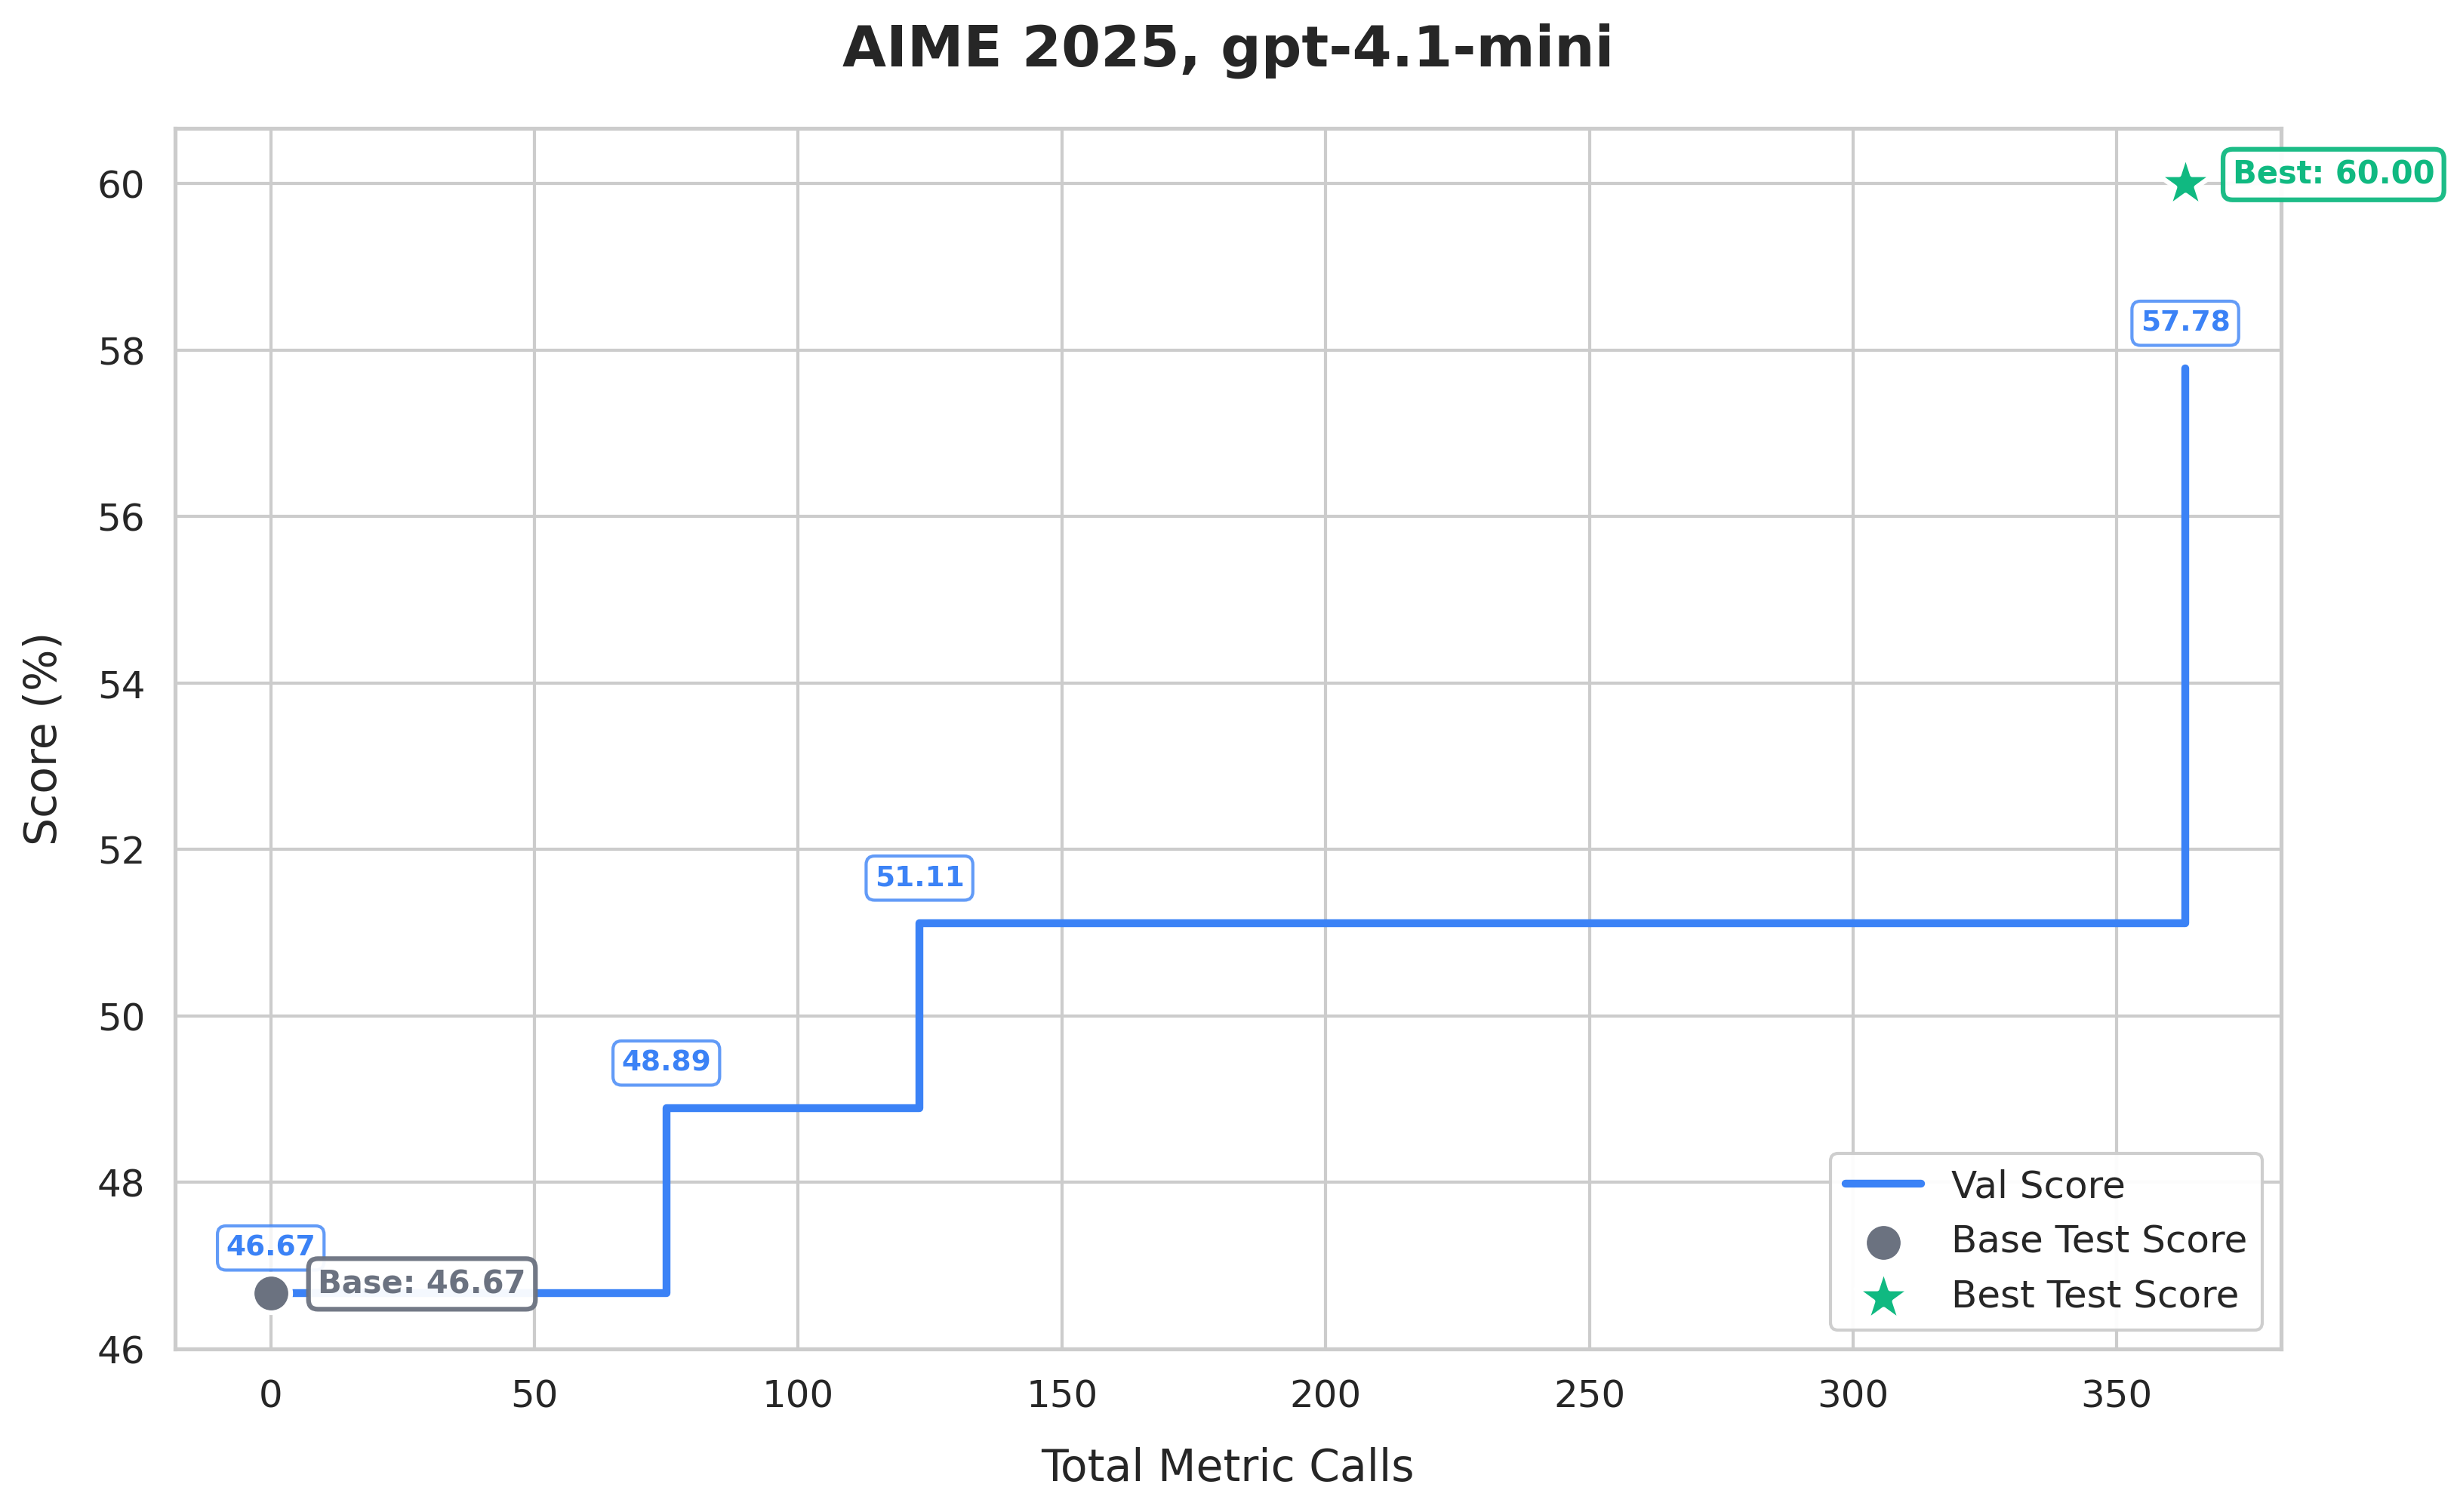
\includegraphics[width=\columnwidth]{figures/aime_results.png}
  \caption{AIME prompt optimization for GPT-4.1-mini. Validation score improves from 46.67\% to 57.78\%; test score reaches 60.00\%.}
  \Description{Line chart showing validation score improving over 350 metric calls. Test accuracy reaches 60\% from 46.67\% baseline.}
  \label{fig:aime}
\end{figure}


\subsection{CUDA Kernel Generation (Multi-Task Search)}\label{sec:cuda}

\textbf{Setup.} We generate CUDA kernels for 31 reference PyTorch operations from KernelBench~\cite{kernelbench2025}, evaluated on a V100 32GB GPU. The 31 problems span diverse operations: matrix multiplications, convolutions, reductions, element-wise ops, and normalization layers. Under the hood, \oa{} evolves the prompt that drives kernel generation; in multi-task mode, insights discovered for one problem (e.g., how to handle memory coalescing) transfer to others automatically through the shared Pareto frontier.

\textbf{\asi{} design.} The evaluator compiles the generated kernel, runs correctness tests (max absolute error vs. PyTorch reference), and benchmarks wall-clock time. \asi{} includes: (i) NVCC compiler errors with line numbers, (ii) correctness test failures with actual vs.\ expected outputs, (iii) relevant CUDA documentation snippets, and (iv) speedup ratio vs.\ the PyTorch baseline.

\textbf{Results.} 87\% of generated kernels match or beat the PyTorch baseline performance; 48\% achieve 10\%+ speedups, and 25\% achieve 20\%+ speedups (Figure~\ref{fig:cuda-results}). The evolved kernels employ techniques such as float4 vectorization, two-pass algorithms (compute statistics, then normalize), warp shuffle reductions, and shared memory tiling. Multi-task mode's advantages are analyzed in \S\ref{sec:multi-ablation}.

\begin{figure}[t]
  \centering
  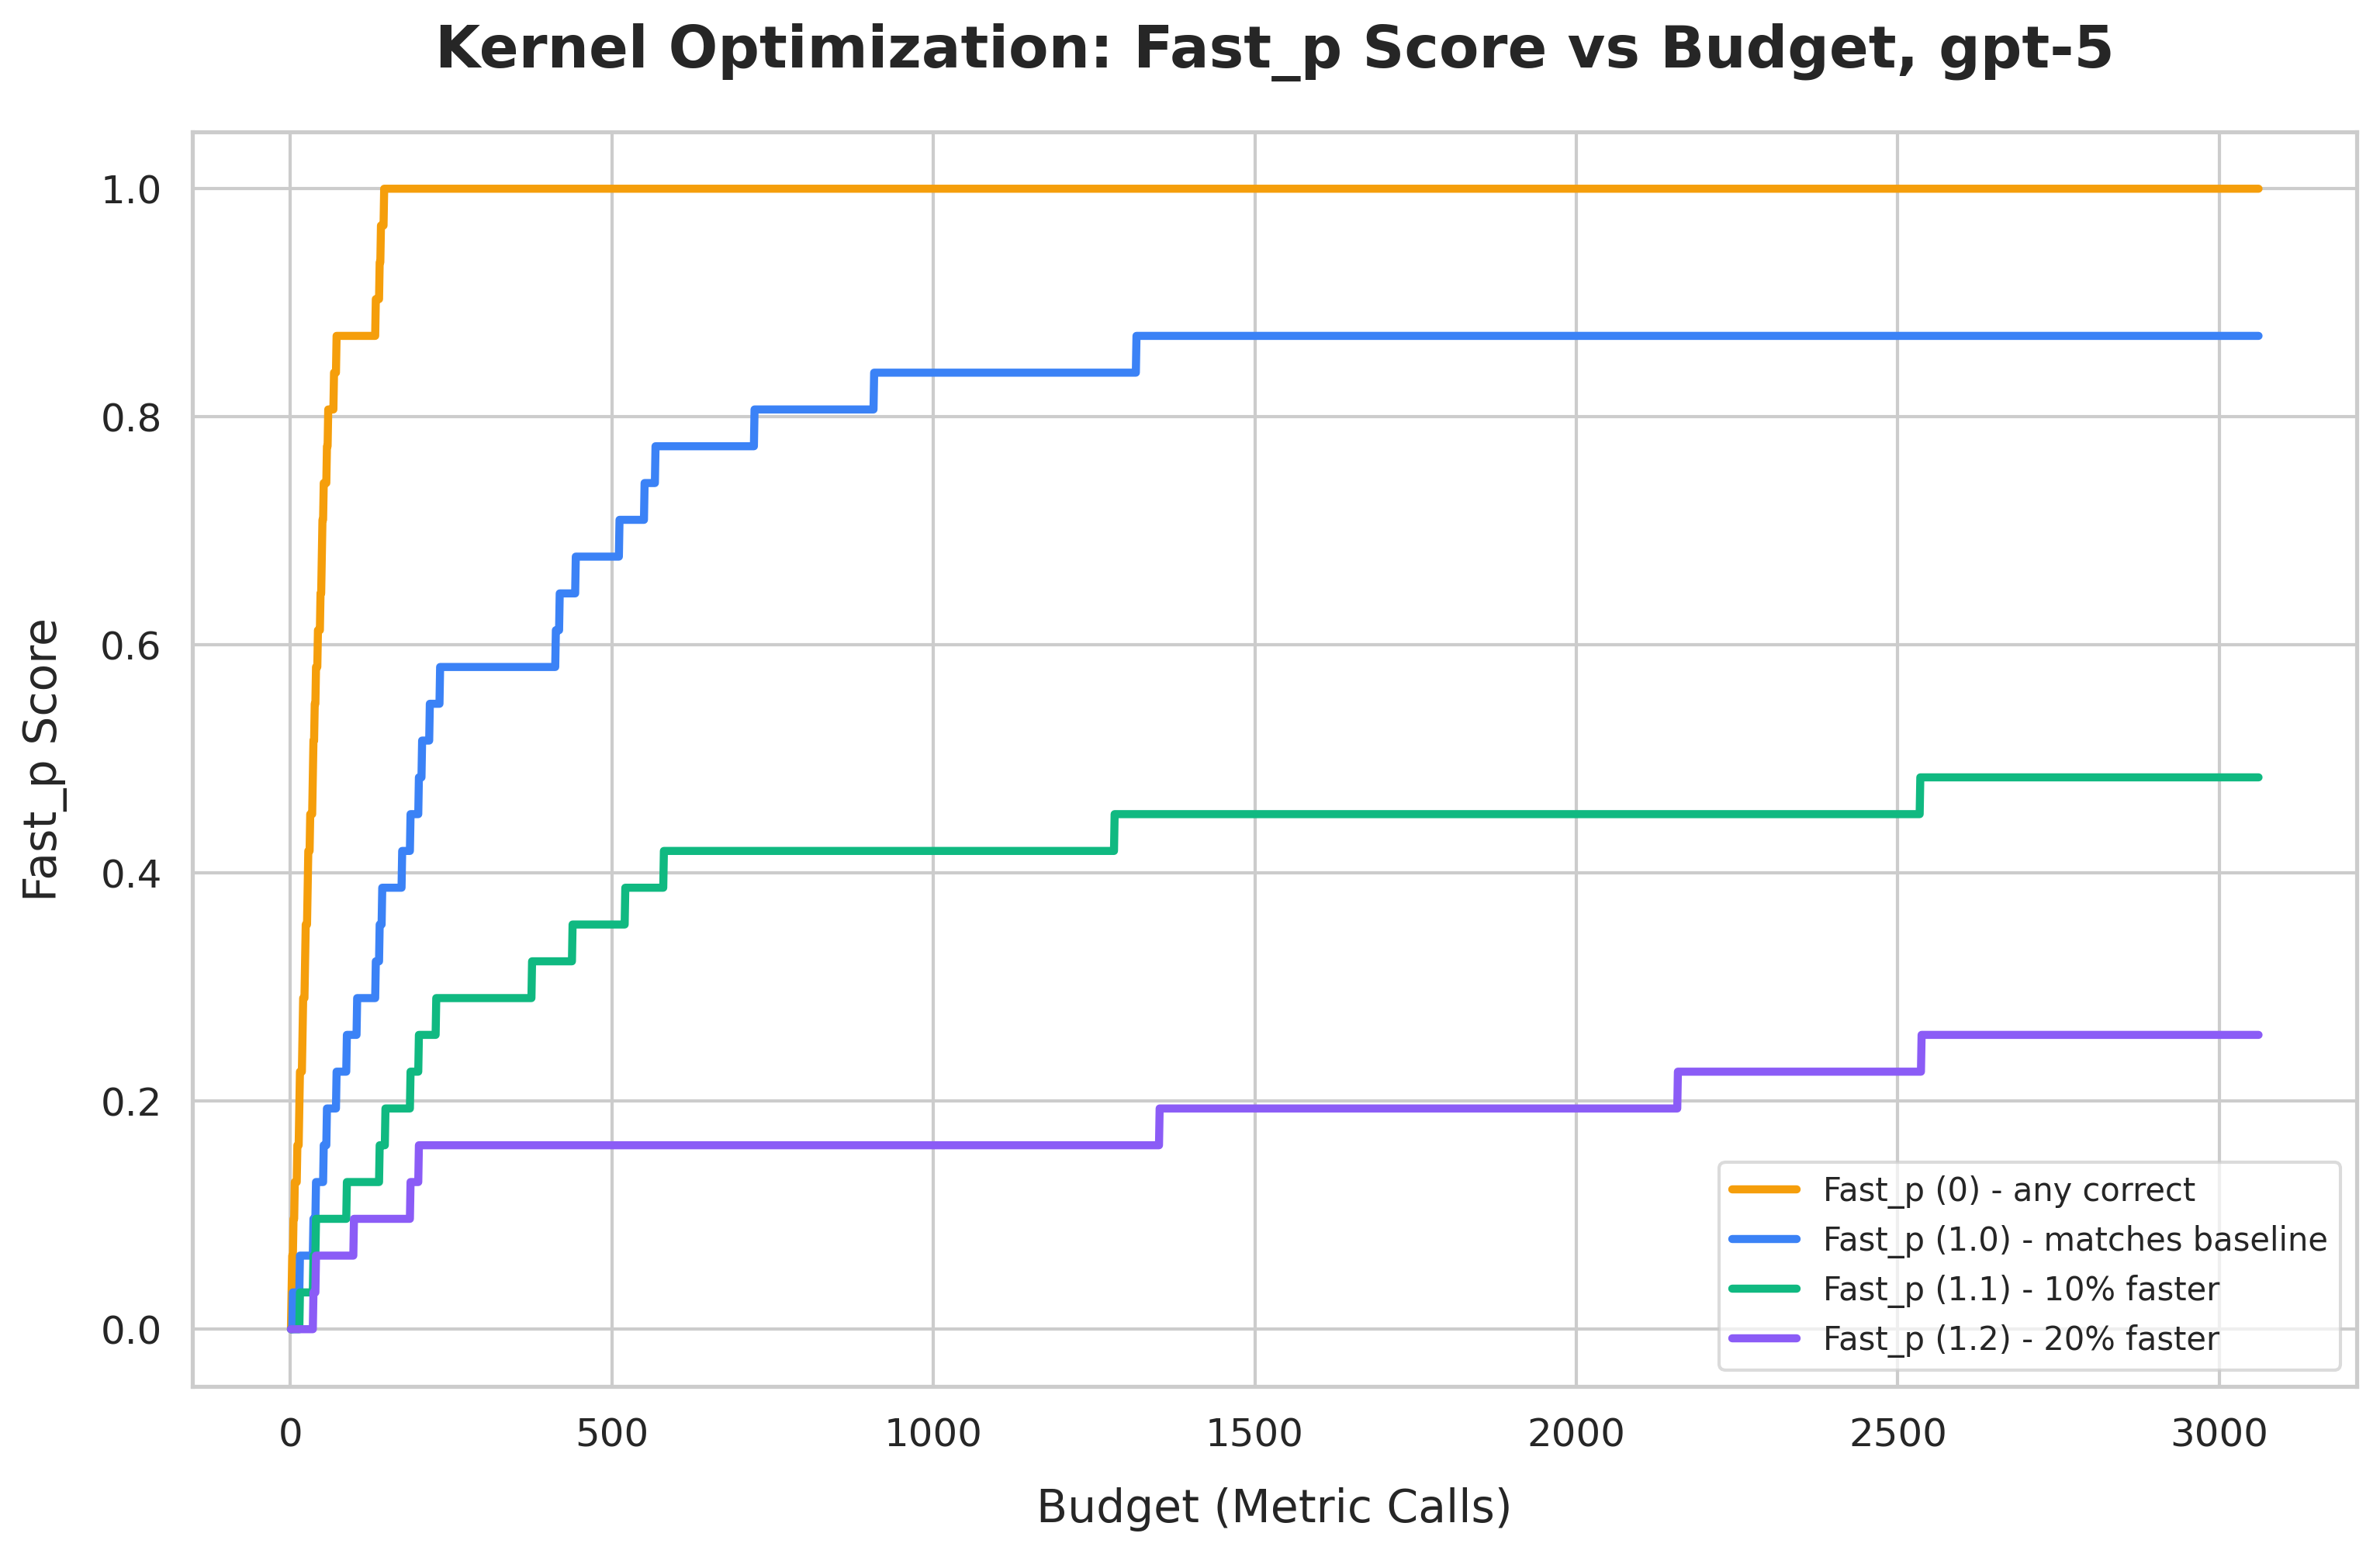
\includegraphics[width=\columnwidth]{figures/kernel_bench_fast_p_score.png}
  \caption{KernelBench results (GPT-5 as proposer). $\text{Fast}_p(s)$: fraction of kernels achieving speedup $\geq s$. 87\% match baseline; 25\% are 20\%+ faster.}
  \Description{Line chart showing Fast\_p at various speedup thresholds. Fast\_p(0)=100\%, Fast\_p(1.0)=87\%, Fast\_p(1.1)=48\%, Fast\_p(1.2)=25\%.}
  \label{fig:cuda-results}
\end{figure}


\subsection{Circle Packing (Single-Task Search)}\label{sec:circle}

\textbf{Setup.} The task is to pack $n{=}26$ circles while maximizing the sum of radii within a unit square. \oa{} optimizes the packing algorithm code; the evaluator executes the proposed packing code, and returns the score plus geometric diagnostics.

\textbf{\asi{} design.} Circle positions, radii, constraint violations, overlap distances, boundary violations, and a rendered visualization of the packing.

\textbf{Results.} \oa{} reaches a score of 2.63598+, outperforming AlphaEvolve's, OpenEvolve's, and ShinkaEvolve's reported solution (Figure~\ref{fig:circle}). The optimized algorithm is a bilevel optimizer: an LP over radii with dual-variable gradients for L-BFGS-B center optimization, augmented by CMA-ES exploration and diverse seeding strategies.

\begin{figure}[t]
  \centering
  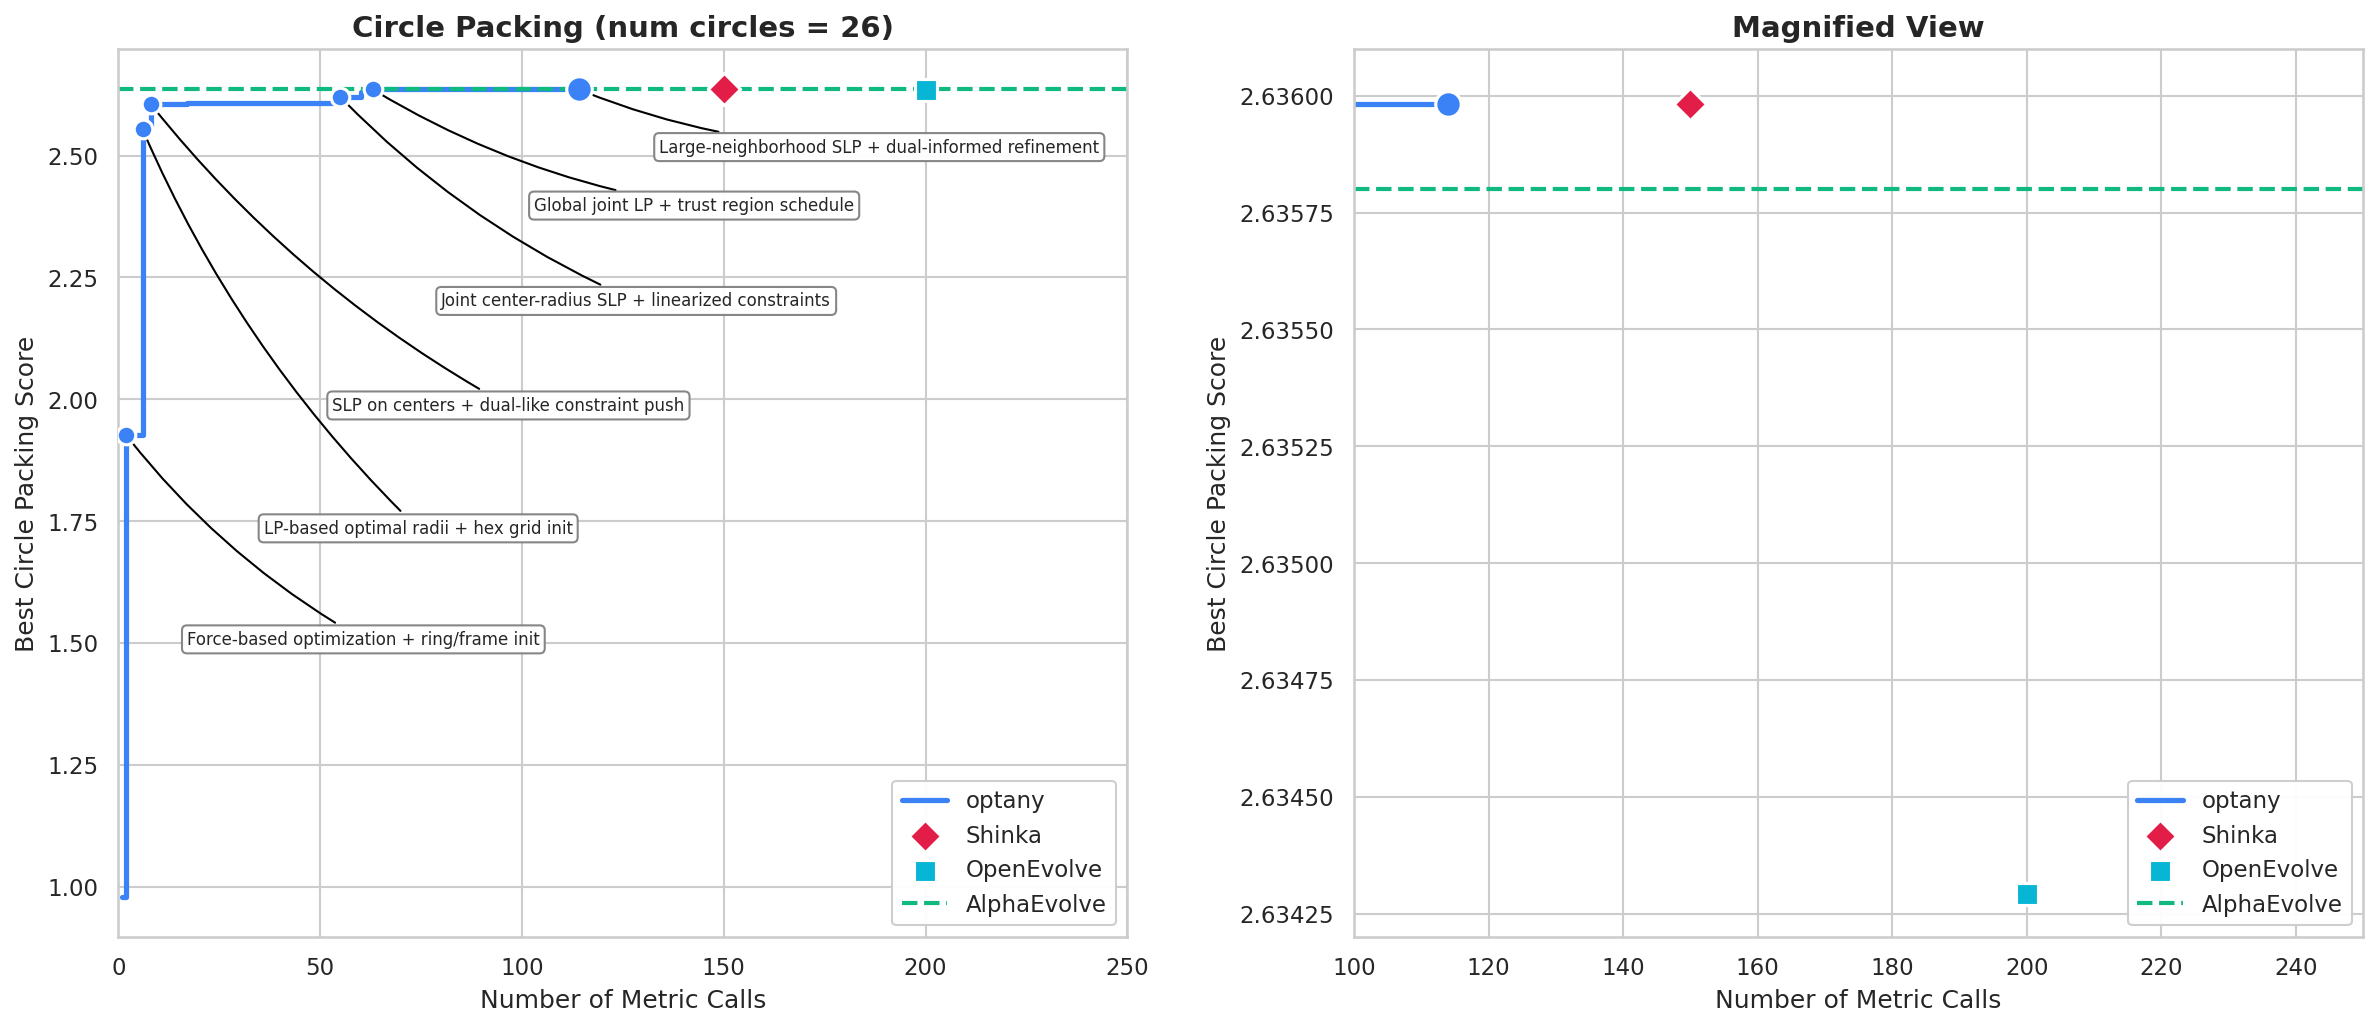
\includegraphics[width=\columnwidth]{figures/circle_packing_annotated3_optany}
  \caption{Circle packing ($n{=}26$). \oa{} outperforms AlphaEvolve's, ShinkaEvolve's, and OpenEvolve's solution, reaching a higher score with fewer evaluations.}
  \Description{Line chart comparing four methods on circle packing. \oa{} reaches highest score around 2.636 with fewer metric calls than alternatives.}
  \label{fig:circle}
\end{figure}

\subsection{Image Generation (Multi-Task Search)}\label{sec:svg-gen}

\textbf{Setup.} The first task is to generate Scalable Vector Graphics (SVG) code to generate an image given a goal defined as a short description that is less than one sentence in length. We do so for three goals. We have one addition setting where we also generate code via \texttt{build123d} to generate CAD and rendering for the CAD. We present the goals in Table \ref{tab:optimization_examples}.

\textbf{\asi{} design.} For the SVG, the evaluator renders the image and then queries a VLM for feedback. For each goal, we define several natural language properties which ask a VLM to rate on a scale of 0 to 100 how well the image aligns with that aspect. During each evaluator call, the VLM is asked to rate one aspect and not all at once hence the \textbf{Multi-Task Search} which allows us to explore the Pareto frontier. In the CAD setting, since we are dealing with 3D objects, we have the evaluator take 3 screenshots equidistant apart and ask the VLM to provide feedback using those images.

\textbf{Results.} We ask five humans (including several independent people) to examine the images created by the CAD and SVG code from a zero-shot attempt and the \oa{} optimized candidates. The images are provided without identification and the humans are asked to simply pick which image they prefer. In all goals, the \oa{} optimized candidates were unanimously preferred over the zero-shot attempts. 

\begin{table*}[t]
    \centering
    \small
    \setlength{\tabcolsep}{8pt}
    \begin{tabular}{p{8.2cm}c c p{3.2cm}}
    \hline
    Goal & \# Visual Aspects & Representation & Model Used in Optimization \\
    \hline
    A pelican riding a bicycle & 12 & SVG & \texttt{Gemini Flash 3.0} \\
    A high-quality 3D unicorn & 4 & CAD & \texttt{Claude Opus 4.6} \\
    An octopus performing on a grand pipe organ & 13 & SVG & \texttt{Claude Opus 4.6} \\
    A sloth steering an excavator through a cinematic quarry at golden hour & 13 & SVG & \texttt{Claude Opus 4.6} \\
    \hline
    \end{tabular}
    \caption{An overview of the various target images (\textit{goals}) from the Image Generation Experiments in \S\ref{sec:svg-gen}. In each experiment, a VLM is used in the evaluator to provide natural langauge feedback and a score between 0 and 100 for a single visual aspect.}
    \label{tab:optimization_examples}
\end{table*}


%% ================================================================
\subsection{Ablation: Multi-Task vs. Single-Task Search}\label{sec:multi-ablation}

To gauge the effectiveness of cross-task learning, we take the 10 problems where multi-task mode performed best and re-optimize each from scratch in single-task mode. We allocate an equivalent per-problem budget to see whether a dedicated single-task run can match the multi-task result.

Figure~\ref{fig:multi-ablation} shows that multi-task mode consistently outperforms single-task search across all speedup thresholds. At the $\text{Fast}_p(1.0)$ threshold (matching baseline performance), multi-task mode solves problems faster and reaches a higher fraction solved. At $\text{Fast}_p(1.2)$ (20\% speedup), the gap widens: single-task mode plateaus early, while multi-task continues improving.

\begin{figure}[t]
  \centering
  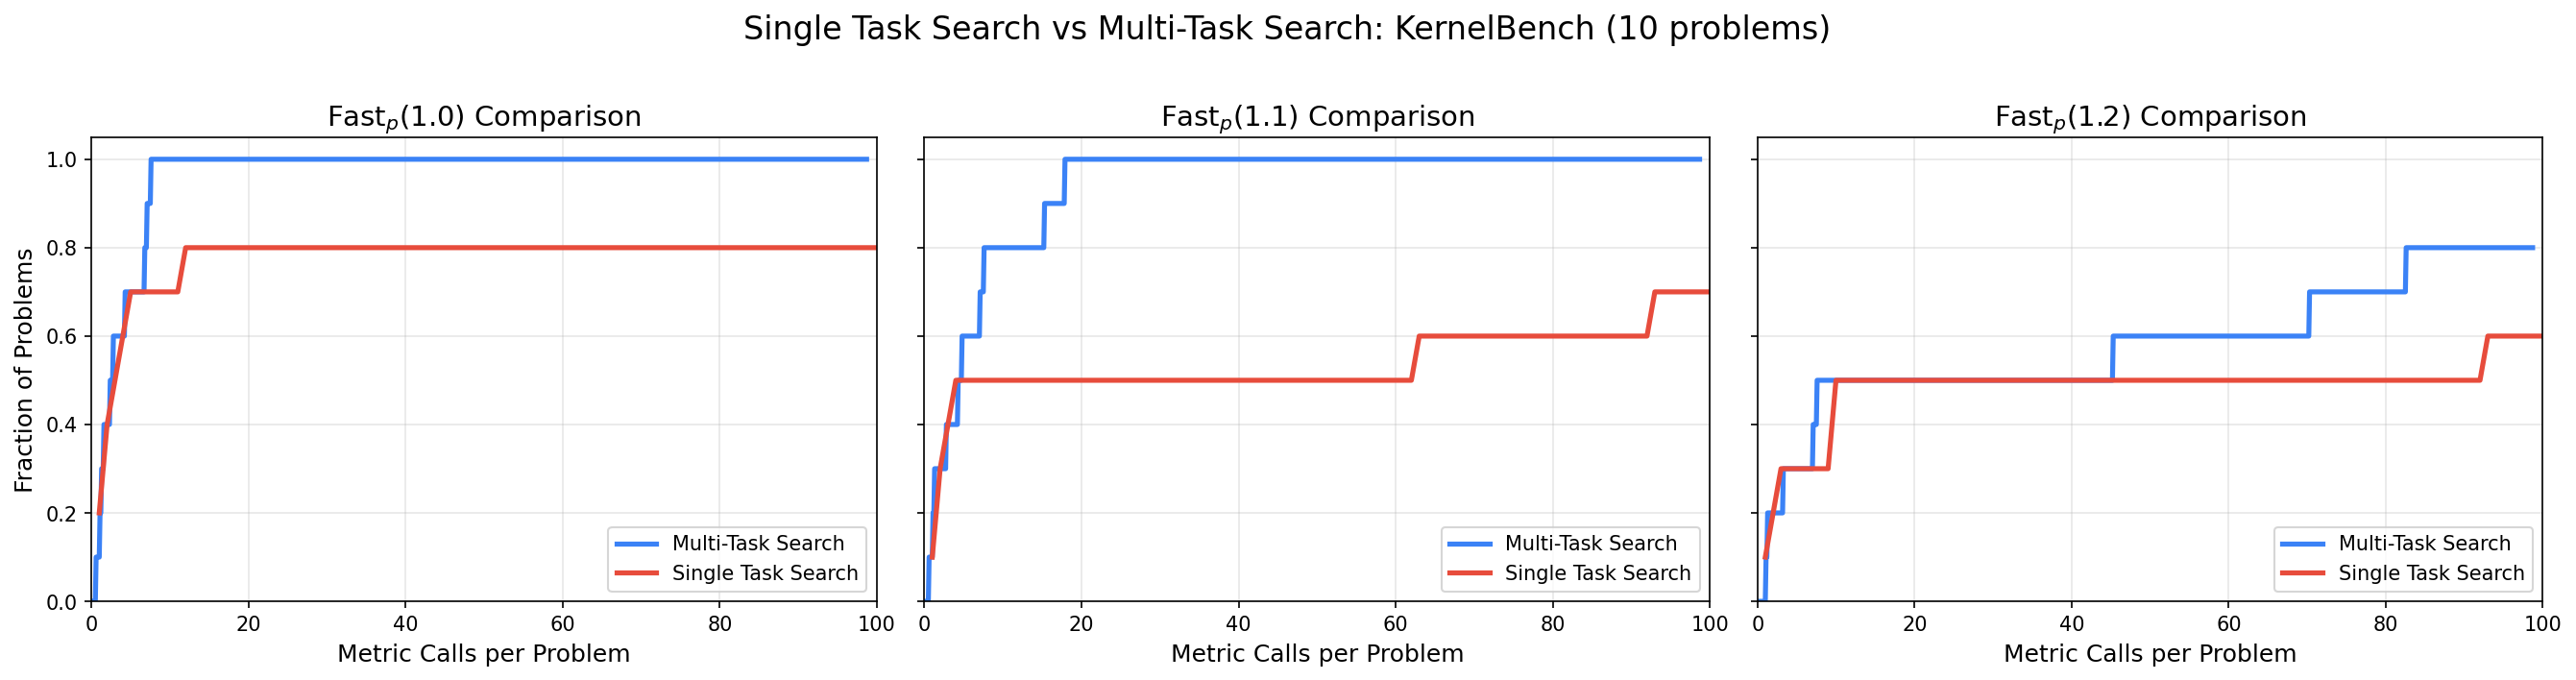
\includegraphics[width=\columnwidth]{figures/kernelbench_single_vs_batch.png}
  \caption{Single-task vs.\ multi-task mode on 10 selected KernelBench problems. Multi-task (blue) consistently outperforms single-task (red) at all speedup thresholds, converging faster and solving more problems.}
  \Description{Three line charts comparing single vs batch mode at F(1.0), F(1.1), F(1.2) thresholds. Batch mode solid lines are consistently above single mode dashed lines.}
  \label{fig:multi-ablation}
\end{figure}

The mechanism is cross-transfer via the Pareto frontier: optimization patterns discovered for one kernel (e.g., vectorized memory access, warp-level reductions) are preserved on the frontier and inform proposals for other kernels. In single-task mode, each problem must independently discover these patterns.

\subsection{Ablation: Side Information}\label{sec:asi-ablation}

To isolate the contribution of \asi{}, we compare \oa{} with and without structured diagnostic feedback (sub-scores) on prompt optimization for the Facility Support Analysis dataset. In the ``with \asi{}'' condition, the evaluator returns per-aspect sub-scores alongside the aggregate score. In the ``without \asi{}'' condition, only the aggregate score is returned.

Figure~\ref{fig:asi-ablation} shows two effects. First, \asi{} accelerates convergence: the ``with \asi{}'' condition reaches a validation score of 0.80 within 100 rollouts, while the score-only condition requires approximately 600 rollouts to reach the same level. Second, \asi{} improves final performance: the test score with \asi{} is 86.32 versus 82.5 without.

\begin{figure}[t]
  \centering
  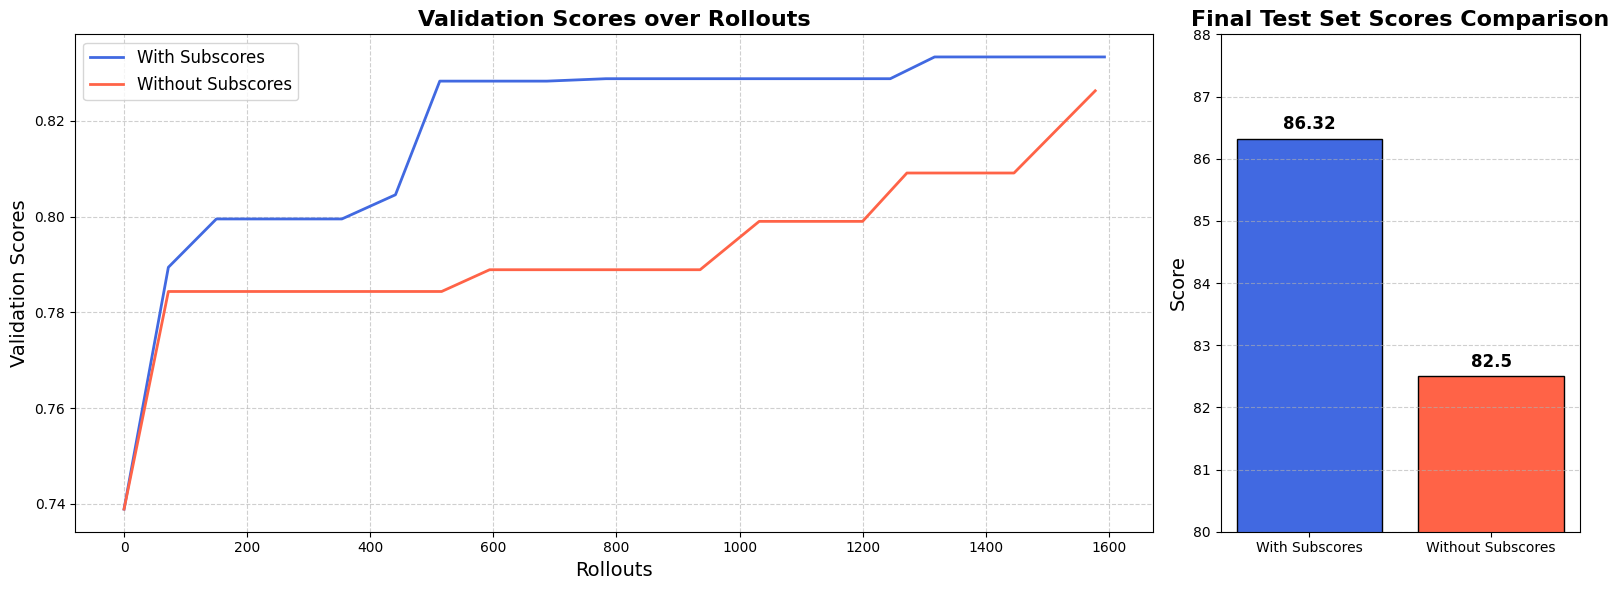
\includegraphics[width=\columnwidth]{figures/with_text_feedback_vs_without.png}
  \caption{Ablation: prompt optimization with vs.\ without \asi{} on the Facility Support Analysis dataset. \asi{} accelerates convergence (left) and improves final test performance (right): 86.32 vs.\ 82.5.}
  \Description{Left: validation score curves showing with-subscores (blue) converging faster than without (red). Right: bar chart showing final test scores 86.32 vs 82.5.}
  \label{fig:asi-ablation}
\end{figure}

Sub-scores provide per-aspect signal: the proposer can identify that a candidate excels at aspect A but fails at aspect B, and target its revision accordingly. Without sub-scores, the proposer receives only ``the overall score improved slightly,'' losing the diagnostic signal that enables targeted improvements.

%% ================================================================
\section{Discussion}\label{sec:discussion}

\paragraph{When does multi-task search help?}
Our experiments reveal that cross-task transfer is most beneficial when problems share underlying optimization patterns but differ in their specifics. CUDA kernel generation exemplifies this: memory coalescing, vectorized access patterns, and warp-level reductions are strategies that apply across operations but manifest differently for each kernel. Multi-task mode discovers these patterns once and transfers them, while single-task mode must rediscover them independently for each problem. We hypothesize that multi-task search will be most effective for code generation tasks where common optimization idioms exist across a family of programs.

\paragraph{The role of \asi{} across domains.}
The \asi{} ablation on prompt optimization demonstrates the value of structured diagnostic feedback, but the mechanism operates differently across domains. For code optimization (CUDA, circle packing), \asi{} primarily surfaces compiler errors and runtime diagnostics that pinpoint exact failure locations. For agent architecture evolution (ARC-AGI), \asi{} provides per-puzzle execution traces that reveal which architectural components are failing. For cloud scheduling, \asi{} exposes the temporal structure of decisions, like when the policy chose SPOT vs. ON\_DEMAND and whether that choice was optimal in retrospect. In each case, \asi{} converts a scalar signal into actionable diagnostic information that enables the proposer to make targeted rather than random improvements.

\paragraph{Artifacts optimized by \oa{}.}
A notable property of the results is the diversity of artifacts optimized through a single interface. The optimized artifacts range across structured system prompts (AIME), agent architectures (ARC-AGI) to 900+ line bilevel optimization algorithms (circle packing). The system discovers qualitatively different solution strategies: multi-stage pipelines with fallback logic (ARC-AGI), provider-aware Steiner tree algorithms (CloudCast), and break-even cost analysis with state tracking (Can't Be Late). Beyond minor refinements of the seed, they represent novel algorithmic ideas arising from the interaction between LLM reasoning and diagnostic feedback.

%% ================================================================
\section{Limitations}\label{sec:limitations}

\oa{} inherits limitations from LLM-based optimization. First, the quality of proposals depends on the proposer LLM's capabilities; weaker models produce weaker candidates. Second, evaluation cost can be high when the evaluator involves expensive operations (e.g., running a full agent on many tasks). Third, the system assumes the artifact is representable as text; optimization of continuous parameters or binary artifacts requires a text-based proxy. Fourth, while multi-task search provides cross-transfer benefits on related problems, the degree of benefit depends on how related the problems are, for example, we find that circle packing does not benefit from multi-task mode. Finally, our \asi{} ablation is conducted on a single prompt optimization task; broader ablations across domains would strengthen the finding.


%% ================================================================
\section{Conclusion}\label{sec:conclusion}

\oa{} demonstrates that a simple declarative interface consisting of seed artifact (or objective), evaluator and optional dataset is sufficient to express and solve diverse optimization problems as an optimization over text artifacts, matching or outperforming purpose-built tools. The key ideas are (1) three unified optimization modes under one API, (2) Side Information as a first-class evaluator contract, and (3) Pareto-based search across metrics and examples. As LLMs become more capable, we expect the range of problems expressible as text optimization to expand further. The \oa{} API is designed to be backend-agnostic: as new optimization strategies emerge, they can be plugged in without changing user code.


%% ================================================================
\begin{acks}
Acknowledgments omitted for double-blind review.
\end{acks}

\bibliographystyle{ACM-Reference-Format}
\bibliography{references}

%% ================================================================
\newpage

\appendix

\section{Use of Generative AI}
The authors made use of Generative AI technologies including ChatGPT, Gemini, Claude and Cursor to generate sections of this Work, including text, tables, graphs, code, etc. The experiment design and details were explicitly the authors' original ideas.

\section{Blackbox Mathematical Optimization}\label{app:optuna}

We additionally evaluate \oa{} in single-task search mode on blackbox mathematical optimization, using the 56-problem EvalSet benchmark~\cite{evalset2018} against Optuna~\cite{akiba2019optuna}. Rather than tuning parameters within a fixed algorithm, \oa{} optimizes the solver code itself, discovering bespoke algorithms for each problem.

With a budget of 8,000 evaluations per problem, \\ \oa{} ties Optuna on 40 problems, wins 7, and loses 9. On 10 selected problems where Optuna struggles with lower budgets (2,000 evaluations), \oa{} finds better solutions on 7 out of 10. The mechanism: Optuna's fixed TPE-CMA-ES pipeline fails in predictable, structural ways (e.g., TPE's per-dimension sampling converges to trap basins; CMA-ES assumes smooth unimodal landscapes). \oa{} tailors the solver to each problem---discovering L-BFGS-B for boundary optima and multi-start search for deceptive traps.


\section{Seedless Mode: 3D Unicorn}\label{app:unicorn}

Every main experiment starts from a seed artifact. Seedless mode (\texttt{seed\_candidate=None}) instead provides only a natural-language objective and lets the LLM bootstrap the first candidate. We demonstrate this on a 3D modeling task: generating a Python script (build123d + pyrender) that produces a 3D unicorn. The evaluator renders multi-view PNGs and asks a VLM to score them, passing images back as \asi{}. Starting from no code, \oa{} iteratively refines geometry, proportions, and anatomical detail, producing a recognizable 3D unicorn that improves substantially over the zero-shot baseline.

\section{Detailed Algorithm}\label{app:algorithm}

\begin{algorithm}[H]
\caption{\oa{}: Core optimization loop}
\label{alg:oa}
\begin{algorithmic}[1]
\small
\Require Artifact $\Phi_0$, evaluator $f$, dataset $\mathcal{D}$, budget $B$
\Require Minibatch size $b$, Pareto set size $n$
\State Initialize candidates $\mathcal{P} \gets [\Phi_0]$
\State Evaluate $\Phi_0$ on $\mathcal{D}$; record per-example scores $S$
\While{budget $B$ not exhausted}
  \State $k \gets$ \textsc{ParetoSelect}($\mathcal{P}, S$) \Comment{Select based on frontier}
  \State $\mathcal{M} \gets$ minibatch of size $b$ from $\mathcal{D}$
  \State Execute $\Phi_k$ on $\mathcal{M}$; collect scores and \asi{}
  \State $\Phi' \gets$ \textsc{Reflect}($\Phi_k$, scores, \asi{}) \Comment{LLM proposes fix}
  \If{$\Phi'$ improves on $\mathcal{M}$}
    \State Evaluate $\Phi'$ on full $\mathcal{D}$
    \State $\mathcal{P} \gets \mathcal{P} \cup \{\Phi'\}$
    \State Update $S$; prune dominated candidates
  \EndIf
\EndWhile
\State \Return $\Phi^* \in \mathcal{P}$ maximizing average score
\end{algorithmic}
\end{algorithm}

Algorithm~\ref{alg:oa} presents the core loop. For single-task search, the ``dataset'' is a singleton and per-example tracking reduces to per-metric tracking. For multi-task search, each dataset element is an independent problem. For generalization, scores on $\mathcal{D}$ guide search while a held-out \texttt{valset} measures generalization. The \textsc{ParetoSelect} subroutine follows GEPA~\cite{agrawal2026gepa}: it identifies non-dominated candidates and samples proportionally to their frontier frequency.

\section{Discovered solutions}
\label{app:discovered_solutions}

We present excerpts of the final optimized artifacts discovered by \oa{} for each domain. 

\subsection{Coding Agent Skills: Bleve Repository}
\label{app:sol-skills}

The following is the optimized \texttt{SKILL.MD} excerpt discovered by \oa{} for the Bleve search library:

\begin{promptbox}[Optimized Bleve Skills (excerpt)]
4) Run tests early and iterate from failures (tests are the bug report)
- Start broad when feasible: `cd /testbed \&\& go test ./...` (or project equivalent).
- Narrow quickly:
  - package: `go test ./path/to/pkg`
  - single test: `go test ./path/to/pkg -run TestName -count=1` (add -v only if needed)
- For panics: follow the stack trace top frame in repo code first.
- For mismatches: use “expected vs got” to locate the producing function and invariants.

...

7) Make minimal, reviewable changes and verify continuously
- Change one behavior at a time; rerun the smallest reproducing test after each change.
- Add focused unit tests when coverage is missing; keep them in the same package and table-driven where sensible (include short words + accented/Unicode edge cases).
- Avoid scratch main.go files in repo root.
\end{promptbox}


\subsection{ARC-AGI Agent Architecture}
\label{app:sol-arc}

The optimized agent grew from a 10-line seed to a 300+ line system implementing a 4-stage pipeline: rule induction via pattern analysis, code generation with \texttt{exec()}-based verification, iterative debugging with up to 2 fix attempts, and structured fallback from code-first to direct LLM prediction.

\begin{figure}[h]
  \centering
  
\includegraphics[width=\columnwidth]{cais_submission/figures/arc_agi_architecture.png}
  \caption{Architecture of the optimized ARC-AGI agent. The system discovers a 4-stage pipeline with verify-then-fallback logic, starting from a naive single-call seed.}
  \Description{Architecture diagram of the optimized ARC-AGI agent showing four stages: rule induction, code generation with exec()-based verification, iterative debugging, and structured fallback.}
  \label{fig:arc-architecture}
\end{figure}


\subsection{CloudCast Routing Algorithm}
\label{app:sol-cloudcast}

The optimized CloudCast algorithm (178 lines) discovers provider-aware Steiner tree routing with egress cost optimization, a qualitative departure from the Dijkstra seed. 

We show the main \texttt{search\_algorithm} function; the full artifact is available in the supplementary material.

\begin{promptbox}[Optimized CloudCast Algorithm (excerpt)]
\begin{lstlisting}[aboveskip=0pt,belowskip=0pt,numbers=none,frame=none,backgroundcolor=\color{gray!5}]
def search_algorithm(src, dsts, G, num_partitions):
    """Optimized Broadcast Routing Algorithm v3.
    Key Optimizations:
    1. Provider-Aware Weighting: biases path finding towards
       intra-provider links to minimize egress.
    2. Pareto-Frontier Candidate Selection: Explicitly keeps
       candidates that offer distinct cost/time tradeoffs.
    3. Diverse Steiner Strategies: Includes MST-like
       approximations for cost and bottleneck-widest
       paths for throughput.
    4. Robust Greedy Allocation: Accurately models bandwidth
       contention across partitions.
    """
    # --- Constants & Configuration ---
    EST_DATA_VOL_GB = 300.0
    EST_INSTANCE_COST_PER_HR = 10.0
    PARTITION_VOL_GB = EST_DATA_VOL_GB / max(1, num_partitions)
    # Sweep parameters for Cost vs Time tradeoff
    alphas = [0.0, 1e-5, 0.001, 0.01, 0.05, 0.1, 0.5, 2.0]
    bw_thresholds = [0.0, 0.5, 5.0, 20.0]
    strategies = ['prim', 'prim', 'furthest', 'random']
    # ... (remaining 140 lines: provider extraction, graph
    #  preprocessing, Steiner tree construction, greedy
    #  allocation, and Pareto-frontier selection)
\end{lstlisting}
\end{promptbox}

\subsection{Can't Be Late Scheduling Policy}
\label{app:sol-cantbelate}

The optimized scheduling policy (110 lines) starts from a simple deadline-check heuristic and discovers three key behaviors absent from the seed: (1) break-even switching cost analysis that avoids costly SPOT$\to$ON\_DEMAND transitions when remaining work is small, (2) persistent spot-unavailability tracking via a counter that detects when SPOT is unlikely to return, and (3) graduated decision thresholds based on slack ratio that become increasingly aggressive as the deadline approaches. We show the core \texttt{\_step} method; the full artifact includes \texttt{reset()} and additional edge-case guards.


\begin{promptbox}[Optimized Can't Be Late Policy (excerpt)]
\begin{lstlisting}[aboveskip=0pt,belowskip=0pt,numbers=none,frame=none,backgroundcolor=\color{gray!5}]
from sky_spot.strategies.strategy import Strategy
from sky_spot.utils import ClusterType

class EvolveSingleRegionStrategy(Strategy):
    def __init__(self, args):
        super().__init__(args)
        self.spot_unavailable_count = 0
        self.consecutive_short_spot_windows = 0

    def _step(self, last_cluster_type, has_spot) -> ClusterType:
        remaining_task_time = self.task_duration - sum(self.task_done_time)
        remaining_time = self.deadline - self.env.elapsed_seconds
        slack = remaining_time - remaining_task_time - self.restart_overhead

        # Track persistent spot unavailability
        if not has_spot:
            self.spot_unavailable_count += 1
        else:
            self.spot_unavailable_count = 0

        # Critical deadline: must use ON_DEMAND
        if remaining_task_time + self.restart_overhead >= remaining_time - 0.5:
            return ClusterType.ON_DEMAND

        slack_ratio = slack / max(remaining_task_time, 1e-6)

        if has_spot:
            if last_cluster_type == ClusterType.ON_DEMAND:
                # Break-even analysis: is switching to SPOT worth it?
                switch_cost = self.restart_overhead * 1.0
                savings_per_hour = 0.7  # OD(1.0) - SPOT(0.3)
                break_even = switch_cost / savings_per_hour
                if remaining_task_time < break_even * 1.5:
                    return ClusterType.ON_DEMAND
                if slack < self.restart_overhead * 3:
                    return ClusterType.ON_DEMAND
            return ClusterType.SPOT
        else:
            if last_cluster_type == ClusterType.ON_DEMAND:
                return ClusterType.ON_DEMAND
            # Graduated thresholds based on slack ratio
            if slack_ratio < 0.1:
                return ClusterType.ON_DEMAND
            if slack_ratio < 0.25 and self.spot_unavailable_count > 10:
                return ClusterType.ON_DEMAND
            if slack_ratio < 0.4 and self.spot_unavailable_count > 20:
                return ClusterType.ON_DEMAND
            return ClusterType.NONE  # Wait for spot
    # ... (remaining 15 lines: reset(), _from_args(),
    #  and additional small-task / tight-deadline guards)
\end{lstlisting}
\end{promptbox}

\subsection{CUDA Kernel: LayerNorm}
\label{app:sol-cuda}

We show the best individual kernel discovered for LayerNorm, which achieves a 3.32$\times$ speedup over the PyTorch baseline. The kernel employs three key techniques absent from the naive implementation: (1) \texttt{float4} vectorization that loads four values per memory transaction, cutting memory overhead by $\sim$4$\times$; (2) a two-pass algorithm (compute statistics, then normalize) that lets the GPU optimize each phase independently; and (3) warp shuffle reductions (\texttt{\_\_shfl\_down\_sync}) for direct register-to-register partial sum accumulation, bypassing slower shared memory paths. This kernel was discovered in multi-task mode, where optimization patterns transfer across the 31 KernelBench problems via the shared Pareto frontier.

\begin{promptbox}[Optimized LayerNorm CUDA Kernel (excerpt)]
\begin{lstlisting}[aboveskip=0pt,belowskip=0pt,numbers=none,frame=none,backgroundcolor=\color{gray!5},language=C++]
__inline__ __device__ float warp_sum(float v) {
    unsigned mask = 0xffffffffu;
    for (int offset = KB_WARP_SIZE / 2; offset > 0; offset >>= 1)
        v += __shfl_down_sync(mask, v, offset);
    return v;
}

__global__ void rowwise_stats_kernel(
    const float* __restrict__ x, float* __restrict__ mean,
    float* __restrict__ inv_std, int64_t B, int64_t M, float eps) {
    int64_t row = blockIdx.x;
    if (row >= B) return;
    const float* row_ptr = x + row * M;

    float thread_sum = 0.0f, thread_sumsq = 0.0f;
    // float4 vectorized loads when aligned
    const float4* row_v4 = reinterpret_cast<const float4*>(row_ptr);
    for (int64_t j = threadIdx.x; j < (M >> 2); j += blockDim.x) {
        float4 v = row_v4[j];
        thread_sum   += (v.x + v.y + v.z + v.w);
        thread_sumsq += (v.x*v.x + v.y*v.y + v.z*v.z + v.w*v.w);
    }
    // Warp shuffle reduction + cross-warp shared memory reduce
    thread_sum = warp_sum(thread_sum);
    thread_sumsq = warp_sum(thread_sumsq);
    // ... (shared memory cross-warp reduction, mean/inv_std output)
}

__global__ void layernorm_affine_kernel(
    const float* __restrict__ x, const float* __restrict__ weight,
    const float* __restrict__ bias, const float* __restrict__ mean,
    const float* __restrict__ inv_std, float* __restrict__ y,
    int64_t B, int64_t M) {
    int64_t row = blockIdx.x;
    float m = mean[row], inv = inv_std[row];
    // Vectorized normalize + affine transform
    const float4* x_v4 = reinterpret_cast<const float4*>(x + row*M);
    float4* y_v4 = reinterpret_cast<float4*>(y + row*M);
    for (int64_t j = threadIdx.x; j < (M >> 2); j += blockDim.x) {
        float4 xv = x_v4[j], wv = w_v4[j], bv = b_v4[j];
        y_v4[j] = {((xv.x-m)*inv)*wv.x+bv.x, ((xv.y-m)*inv)*wv.y+bv.y,
                    ((xv.z-m)*inv)*wv.z+bv.z, ((xv.w-m)*inv)*wv.w+bv.w};
    }
}
// ... (remaining 80 lines: host function, input validation,
//  thread/block configuration, Python module wrapper)
\end{lstlisting}
\end{promptbox}

\subsection{Circle Packing Algorithm}
\label{app:sol-circle}

The evolved circle packing algorithm (480+ lines) is a bilevel optimizer that jointly optimizes circle centers and radii for $n{=}26$ circles in a unit square. Starting from a simple greedy packing seed, the system discovers a multi-stage architecture: (1) an LP over radii with dual-variable sensitivities that provide exact gradients for center optimization, (2) L-BFGS-B over centers using these LP-derived gradients, (3) block SLP trust-region boosts targeting the worst-performing circles, (4) CMA-ES global exploration with automatic restarts, and (5) aggressive relocation of smallest circles to edges and corners. The algorithm also employs six diverse seeding strategies (hexagonal, uniform, edge-ring, farthest-point, corner-spokes, and edge-biased hex) to avoid local optima. We show the main entry point and key optimization components.

\begin{promptbox}[Evolved Circle Packing Algorithm (excerpt)]
\begin{lstlisting}[aboveskip=0pt,belowskip=0pt,numbers=none,frame=none,backgroundcolor=\color{gray!5}]
def main(timeout, current_best_solution):
    """Bilevel L-BFGS with exact LP sensitivities +
    SLP block boosts + CMA/Evolution fallback"""
    n = 26
    # LP for optimal radii given centers; returns duals
    def solve_radii_lp(centers, need_duals=False):
        # Boundary constraints: r_i <= min(x_i, 1-x_i, y_i, 1-y_i)
        # Pairwise constraints: r_i + r_j <= ||c_i - c_j||
        # Objective: maximize sum(r)
        res = linprog(c_obj, A_ub=A_ub, b_ub=b_ub, ...)
        return r, success, {'dual': res.ineqlin.marginals}

    # Gradient from LP duals: sensitivity of sum(r) to centers
    def gradient_from_duals(centers, dual_vec):
        # Boundary: g[i,0] += (dual_left - dual_right)
        # Pairwise: g[i] += lambda_k * unit_vec(i->j)
        return g

    # Bilevel: L-BFGS-B over centers, LP over radii
    def lbfgs_bilevel(centers_init, max_iters=300):
        def f_and_g(flat):
            r, _, info = solve_radii_lp(centers, need_duals=True)
            g = gradient_from_duals(centers, info['dual'])
            return -score, -g.reshape(-1)
        minimize(f_and_g, method='L-BFGS-B', bounds=bounds)

    # Block SLP: trust-region moves on worst circles
    def block_slp_boost(centers, rounds=4, k=10, delta=0.18):
        # Jointly optimize dx, dy, r via linearized LP
        # Focus on smallest radii + highest gradient circles

    # CMA-ES global exploration over center positions
    # 6 seeding strategies: hex, uniform, edge-ring,
    #   farthest-point, corner-spokes, edge-biased hex

    # Pipeline: seed evaluation -> L-BFGS bilevel ->
    #   block SLP boost -> CMA-ES -> relocate worst ->
    #   evolutionary exploration -> final SLP polish
    # ... (remaining 350 lines: seeding, CMA-ES, relocation,
    #  evolutionary exploration, final polish)
\end{lstlisting}
\end{promptbox}

\begin{figure*}[p]
    \centering

    \textbf{Zero-shot}\hspace{0.22\textwidth}\textbf{\oa{}}

    \vspace{0.4em}

    
\includegraphics[width=0.495\textwidth,height=0.225\textheight,keepaspectratio]{cais_submission/svg/pelican_zero_shot.png}
    \hspace{0.01\textwidth}
    
\includegraphics[width=0.495\textwidth,height=0.225\textheight,keepaspectratio]{cais_submission/svg/pelican_optany.png}

    \vspace{0.35em}

    
\includegraphics[width=0.495\textwidth,height=0.225\textheight,keepaspectratio]{cais_submission/svg/octopus_zero_shot.png}
    \hspace{0.01\textwidth}
    
\includegraphics[width=0.495\textwidth,height=0.225\textheight,keepaspectratio]{cais_submission/svg/octopus_optany.png}

    \vspace{0.35em}

    
\includegraphics[width=0.495\textwidth,height=0.225\textheight,keepaspectratio]{cais_submission/svg/sloth_zero_shot.png}
    \hspace{0.01\textwidth}
    
\includegraphics[width=0.495\textwidth,height=0.225\textheight,keepaspectratio]{cais_submission/svg/sloth_optany.png}

    \vspace{0.35em}

    
\includegraphics[width=0.495\textwidth,height=0.225\textheight,keepaspectratio]{cais_submission/svg/unicorn_zero_shot.png}
    \hspace{0.01\textwidth}
    
\includegraphics[width=0.495\textwidth,height=0.225\textheight,keepaspectratio]{cais_submission/svg/unicorn_optany.png}

    \caption{Qualitative comparison between zero-shot generations (left) and OptimizeAnything candidates (right) across four example tasks. Optimization consistently improves many visual aspects including composition, structure, detail, and overall visual quality. In our human study, all participants preferred the \oa{} generated images.}
    \label{fig:appendix_zero_shot_vs_optany}
\end{figure*}



\end{document}
